\documentclass[fontsize=14pt,paper=a4,pagesize=auto]{report}
\usepackage[nottoc]{tocbibind}
\usepackage{geometry}
\usepackage{lmodern}
\usepackage[english]{babel}
\usepackage{blindtext}
\usepackage{microtype}
\usepackage{longtable}
\usepackage{multirow}
\usepackage{graphicx}
\usepackage{threeparttable, floatrow}
\newsavebox\mysavebox
\usepackage{booktabs}
\usepackage{notoccite}
\usepackage{chemist}
\usepackage{afterpage}

\usepackage{xcolor,comment, subfiles, graphicx, caption, longtable, subfig, fancyhdr}
\usepackage{float} %Used to force image to appear in the section in which it's declared
\usepackage[colorlinks=false,
            allbordercolors={0 0 0},
            pdfborderstyle={/S/U/W 1}]{hyperref}
\usepackage[parfill]{parskip}
\usepackage{siunitx}
\usepackage[utf8]{inputenc} 
\usepackage[T1]{fontenc} 
\usepackage{amsmath}
\setcounter{tocdepth}{2}



\begin{document}

\begin{titlepage}
	\centering
	
\includegraphics[scale = 0.20]{images/polimi.jpg}\par
	{\Large
		Politecnico di Milano\par
		Scuola di Ingegneria Civile,Ambientale e Territoriale\\
		Master in Geoinformatics\par}
			\vspace{0.5cm}
	{\huge\bfseries
		Feature Selection for Explainable Machine Learning Models\\\par}
	\vspace{1cm}
	{\Large
		{\scshape Bresciani} Matteo\par}
	\vfill
	Referent professor: {\scshape Brovelli} Maria Antonia\par
	\vfill
% Bottom of the page
\end{titlepage}




\begin{abstract}
\addcontentsline{toc}{chapter}{Abstract}

The arrival of big data from heterogeneous sources has had an enormous impact also on environmental studies, including air pollution analysis.\\
At the same time, techniques such as \gls{ml} have increasingly become a standard approaches to make predictions. But with data sets with large samples and covariates, AI models could be more complex to be interpreted and explained.\par
One machine learning issue is that models are usually “black box”: systems of which output are not fully understandable by humans. \\
It should be important to interpret the prediction, especially for critical decisions such as healthcare and policy making.
A way to interpret models for better reliability is to compare feature importance: giving a hierarchy of features could be very useful to detect the most influential variables.\par
This thesis work aims at contributing to the preprocessing phase that is performed for ML models, considering it essential before model training.\\
The challenge of this work is to propose an approach based on the concept of finding the best potential predictive variables with feature selection.\\
The advantage of using it is that the selected features helps reduce redundancy and increase the interpretability of subsequent predictive models.
In detail, this thesis presents a set of tools to preprocess data and select variables with filter, wrapper, and embedded feature selection methods.\par
This approach has been applied in a case study of the D-DUST project, which aims to analyze the impact of intensive farming activities on air quality in the Lombardy region (Northern Italy).\\
Some ML models predictions of air pollutants concentrations are also developed to compare the contribution to the accuracy and interpretability of the results.\\
The experimental results obtained with different feature selection  and resolutions are analyzed and compared with reference results available in the scientific literature.
\\
\\
\end{abstract}
\tableofcontents

\chapter{Introduction}
Today, we have to deal with new technologies such as the internet, GPS or satellite platforms, which provide us numerous and large samples of data.\\ 
The data growth in the last decades implies a demand for not only a better collection and storage of data but also a way to extract relevant information and discard eventually the ones which are useless, dirty or wrong.\par
In this scenario, a set of techniques of preprocessing such as data cleaning and transforming is required in order to extract knowledge from vast datasets \cite{garcia2016big}.
\par
For example, in the last years, exponential growth of spatial data occurred thanks to devices and instrumentation such as satellite platforms and ground sensor stations. \\
One usage is to address them towards sustainable development activities through models and tools in order to improve our environment. \\
Indeed, Big Data is having a crucial relevance in reaching the target of United Nations’ Sustainable Development Goals  \cite{zhang2019orchestrating}.
One critical phenomenon that puts risks on the 'Good health and well-being' and 'Climate action' goals is air pollution.\\
Indeed, air pollution is nowadays considered one of the world's largest environmental health risk \cite{fuller2022pollution}.\\
Science demonstrated that deterioration of ambient air quality, due to the growing concentration of pollutants in the atmosphere, has caused a significant increment of deaths in the world.\par  
Pollutants such as particulate matter, ozone, carbon monoxide and ammonia cause respiratory diseases and are important sources of mortality.
Almost the entire global population (99\%) breathes air that exceeds WHO air quality limits and threatens their health \cite{WHOreport}.\newline
In Europe, the air is becoming cleaner, but persistent pollution, especially in cities, is damaging the health of people. One of the last reports, based on the European Environment Agency (EEA), shows that exposure to air pollution caused around 500,000 early deaths in the European Union (EU) in 2018  \cite{european2018air}.\par
One of the most harmful pollutants is \gls{pm}, which can penetrate your lungs or even your bloodstream.\newline 
Particle pollution includes PM10 and PM.25, with less than, respectively, 2.5 and 10 micrometers diameters.
Most particles come from other contaminants such as sulphur dioxide and nitrogen oxides, which are pollutants emitted from power plants, industries and automobiles.\par
However, a significant source of PM is one generated by intensive farming \cite{burkart2007diffuse}.
In particular, this is a relevant issue in the Po Valley, where intensive agricultural activity is highly employed.\\
In this context, human civilization is trying to limit pollution and improve the environment with the use of technology.\newline
Technology is helping to clean up air pollution, with data-based solutions helping make our cities healthier places to live.\newline
Monitoring, analyzing and predicting air quality in urban areas is one of the tools to cope with the climate change problem.\par
The advent of modern Artificial Intelligence (AI) techniques such as \gls{ml} can be considered as new possibilities for researchers to find solutions to various problems affecting air quality and climate change.
\\  
Data have to be coded so that they may be easily parsed by the machine. 
Indeed, data in the real world is often dirty with inconsistencies, noise, and missing values since are aggregated from different sources. So it's important to improve the data quality by removing redundant and wrong pieces of data.\\
In addition to data cleaning, it is essential that the data used for the training in \acrshort{ml} models are appropriate, by discarding eventual confounding or improper data.\\
A feature selection is required for this purpose, since helps to choose the most considerable variables.\par
My work is focused in detail on this last step, in which I also tried to interpret, by seeing the results, how each factor affects the target variable, which in my case study describes pollution phenomena related to agriculture.\\
The following case study is part of the \gls{d-dust} project which aims to detect factors that contribute more to agricultural pollution (PM2.5 and ammonia) with also a reasonable explanation from the literature.\\
The D-DUST project, funded by Fondazione Cariplo’s ‘Data Science for Science and Society’ call for proposals, counts on Politecnico di Milano, \gls{dica} as the lead partner.\newline
D-DUST aims to provide information on the impact of agricultural and livestock activities on pollutants in the Po Valley (North Italy).\\
Data from ground sensors are combined with observations provided by satellite platforms and, using data science techniques such as machine learning and geostatistical models, support the monitoring of farming-related PM.\\
Indeed, D-DUST aims to verify the impact of this integration for PM monitoring and prediction. 
The merge of data from these two different sources could help the implementation of more accurate predictive models, thanks to the sampling accuracy of the ground sensors and the granularity of the satellite observations.\\
Combination of traditional measurements from ground sensors with the satellites observations is considered nowadays a new monitoring approach \cite{de2018modelling}.\\
The last target of the project is to provide data-driven best-practices to policymakers, farming operators and citizens in order to minimize the production processes' effects on air quality.\par
In this thesis, the approach applied to this case study by means of the selection of the most remarkable covariates that impact pollutants (such as PM2.5 and NH3) will contribute in D-DUST for modelling phase.\\
In the next chapter of my report, I will show the tools developed and the strategy chosen to reach this goal. 
This is the content of the next chapters:

\begin{itemize}
  \item \autoref{chap:background} (\textbf{Background and state of art}): it describes the scenario in which my thesis work takes place, referring in particular to the state of the art;
  \item \autoref{chap:Overview} (\textbf{Overview}): it shows the main steps I take in my work;
  \item \autoref{chap:case} (\textbf{Case Study and Data Modelling}): it's focused on the case study by explaining each step taken in detail, for both the feature selection and modelling part;
 \item \autoref{chap:res} (\textbf{Interpretation of the results}): it's focused on the results achieved in the case study (both feature selection and models);
 \item \autoref{chap:conclusion} (\textbf{Conclusions}): it summarises the findings through the results obtained and aims to display future opportunities.  
\end{itemize} 

\chapter{Background and state of art}
\label{chap:background}
In this chapter, I'm going to contextualize the state of the art of my research work. 
Besides, I'll explain about the target to reach and the solution applied.\par
In our times lots of businesses use Big Data for analysing and providing actionable knowledge.\\
Big Data is defined as large data sets collected from different sources such as applications, social networks and websites.\\
For this, we are seeing nowadays a rapid growth of them, which causes a rise of redundancy and corrupted data.\\
The next consequence will be an accuracy reduction if models are built from them.\\
Data must be pre-processed before training, to reduce overfitting and improve the accuracy of the final model.\par
Another aspect to take into consideration is that a \acrshort{ml} model trained with so many features it would be a black box, in which a lack of interpretability could not be able to explain the decisions taken by the \gls{aii}.\\
So it's needed to care about interpretability to discard eventually confounding variables which can suggest there is a correlation when in fact there is not, even if the model's accuracy is extremely high.\\
For example, a new paper by Alex DeGrave et al. \cite{degrave2021ai} shows that a Deep Learning model trained with improper data was taking shortcuts in COVID-19 detection on radiographs due to the position of certain markers rather than on the actual radiograph.
Another common example of this is the confounding correlation between the number of shark attacks and the ice cream sales shown in Figure \ref{fig:shark}.\newline
\begin{figure}[H]
    \centering
    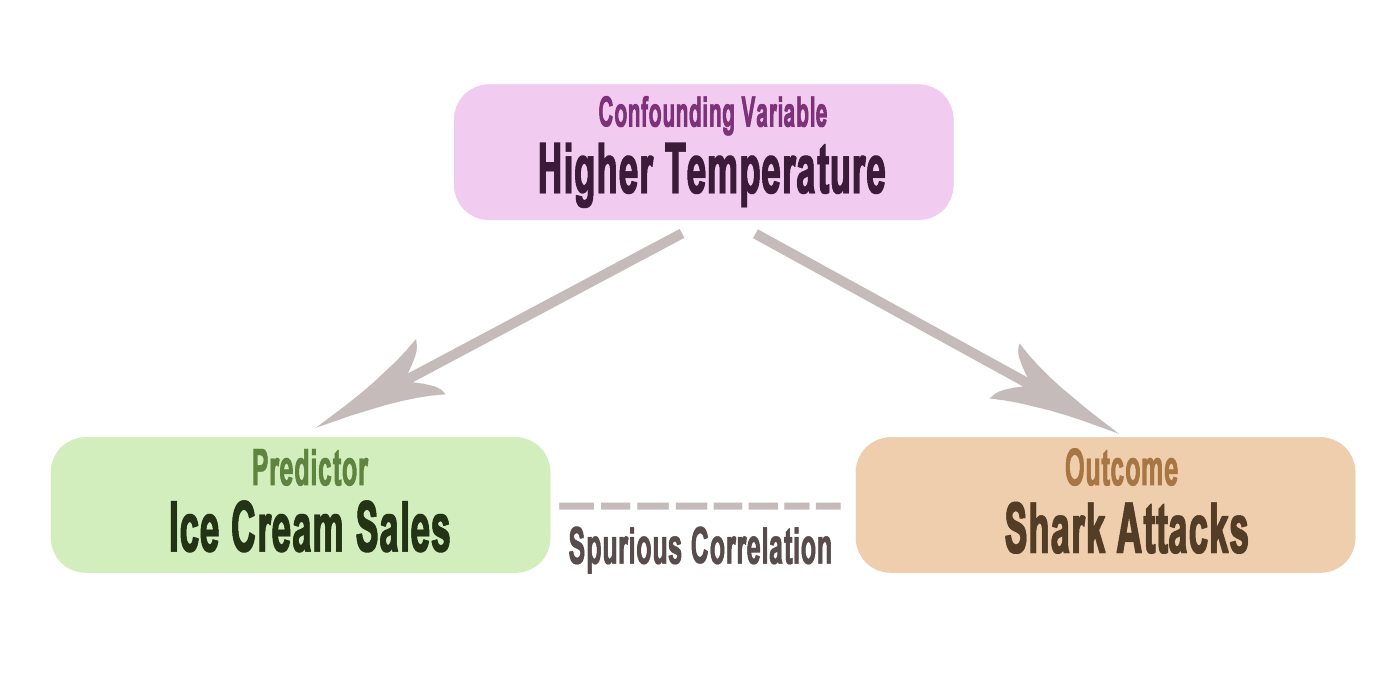
\includegraphics[scale=0.25]{images/confounding.png}
    \caption{The following picture \cite{shark-icecream} highlight how there's no direct relationship between shark attack and ice-cream sales. Instead, they're both caused by a third factor (High temperature) \cite{siegel2019ice}.}
    \label{fig:shark}
\end{figure}
Therefore, the key to increase interpretability of a given model is to wonder if given factor should drive the final decision.\par
In this context, in which the black-box nature of \acrshort{ml} algorithms raises ethical and judicial concerns inducing a lack of trust \cite{9141213}, \gls{xai} aims to create a model fully interpretable.\\
Before the advent of XAI, the scientific community was focused on the predictive power of algorithms rather than the understanding behind these predictions.\\
This need for reliable high performing models led to XAI, a field focused on the interpretation of how AI systems take decisions.
This issue of interpretability and clarity is becoming increasingly significant nowadays. \\
This is consistent with what could be found by searching in Google Trends, where the trend of 'Explainable Artificial Intelligence' grew up in the last 3 years, while the curve of 'AI' seems to have reached a saturation state (Figure \ref{fig:AI_XAI}).\\
In this work, the focus is on model interpretability instead of explainability, even if in literature there are references that describe them in the same way.
Interpretable Artificial Intelligence (or Interpretable Machine Learning) helps to understand how \acrshort{ml} algorithms make prediction, with the use of feature selection methods to clarify the model decision.\par
Feature selection can provide relevant explanations by quantifying the influence of each independent variable with a score.\\
To do that, before developing a predictive model, feature selection is a necessary step to reduce the number of input variables. \newline
Nowadays, with the large volume and variety in Big Data, FS is increasingly becoming an essential preprocessing step in machine learning algorithms \cite{kamolov2021feature}.\\
It is desirable to both reduce the computational cost of modelling and, in some cases, to improve the performance of the model.\newline
\begin{figure}[H]
    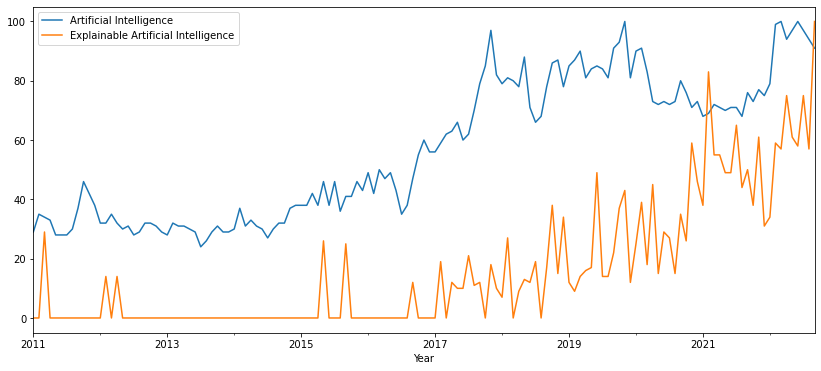
\includegraphics[scale=0.50]{images/AI_XAI.png}
    \caption{This plot is provided by Google Trends in which are shown the scores obtained by 'Artificial Intelligence' and 'Explainable Artificial Intelligence' trends in the period between 2011 and 2022. In this work, the focus is on model interpretability instead of explainability, even if in literature there are references that reported them in the same way.}
    \label{fig:AI_XAI}
\end{figure}
\bigbreak
Inside the D-DUST project, this step aims to provide a weighted score of each environmental variable concerning the pollutants emitted by intense agriculture through regression predictive modelling. Then, scores will be interpreted with findings in literature to confirm them.
Due to the fact that there is no best feature selection techniques, I performed and combined different supervised methods. 
\\
According to the above, my work comes on this scenario, having the aim to preprocess geospatial data in order to highlight the most weighted input variables that affect the pollutants related to intense agriculture and farming.\par
In the next chapter, the FS procedure will be described in detail.


\chapter{Overview}
 \label{chap:Overview}
In this chapter I explain each step taken during the pre-processing phase, by illustrating in details each step taken and tool used. \newline
\par
My work is focused on the first phase of a data analysis procedure which is the pre-processing.
Data pre processing (or data preparation) is the process of transforming raw data into a suitable format for modelling. 
Indeed, raw data is in most cases incomplete and noisy.\par
Nowadays, dealing with big amount of information, the probability of incorrect data is higher without a proper data pre-processing.
Only high-quality data can generate accurate models and predictions. \par
The view and quality of data is very relevant before running any analysis.
Hence, it’s crucial to process data with the best possible quality before training them with artificial intelligence, and machine learning predictive models.\par
\section{Data Collection}
Data collection is the process of gathering information in variables of interest for answering relevant questions. \newline
Relevant data is gathered from their sources and merged in data structures (such as Dataframes). In our work, data come from fixed ground-sensor, satellite-based platform, models and map layers. In this phase are processed (mostly) numerical and categorical data. 
\section{Data Cleaning}
\label{sec:Data cleaning}
Data has to be prepared in accordance with the supervised feature selection.
Data cleaning aims to fix problems or errors in messy data. There are many reasons data may have incorrect values, such as being corrupted, duplicated or invalid. \newline
This could be done by removing rows or columns. Alternately, it might involve replacing observations with new values. \newline
For doing this, I present this solution in sequence, using methods provided by Pandas library:
\begin{itemize}
\item Drop of samples having target variable with NaN value;
\item Drop of columns (values assumed by each covariates) having at least a NaN value;
\end{itemize}
\subsection{Remove of variables with low variance}
An approach for removing columns is to consider the variance of each column variable. The variance is a statistic representing the expected value of the squared deviation from the mean $\mu$ of a given variable X. 
\begin{equation}
  Var(X) = E[(X-\mu)^2]
\end{equation}
The variance can be used as a filter for identifying columns to be removed from a given data set. 
Using a feature with low-variance only adds complexity and noisy to the feature selection and the predictive.\newline
In order to do that, I performed VarianceThreshold method from the scikit-learn library. In this way, features under a certain variance threshold value should be meaningless and consequently discarded by its dataset. 
\section{Data Transformation}
Data need to be scaled. As a matter of fact, each feature in our data has varying degrees of magnitude, range, and units. This is an issue for machine learning algorithms because of highly sensitive to these features. 
Having input variables with different units (e.g. ug/m\textsuperscript{3}, °C, hours or mol/m\textsuperscript{2}) implies data at different scales. This could raise the difficulty of the problem being modelled. \newline
Hence, a common scale through Normalization or Standardization is needed in order to improve the data quality.\newline
Many ML and regression algorithms perform better when numerical input and output variables are scaled to a common standard range. \newline
For instance, it's proved that neural networks trained with scaled data performs better in terms of MSE \cite{shanker1996effect}.
In this step, two type of transformation have been done:
\subsection{Standardization}
The most common data transformation is to centre and scale the each variable values. In order to do that, the average value is removed from all the values. As a result of centring, the predictor will have a zero mean.\cite{kuhn2013applied}
Standardization consists in rescaling data following a Gaussian distribution of values with mean equals to 0 and standard deviation equals to 1:
\begin{equation}
  Z = \frac{X-\mu}{\sigma}
\end{equation}
\begin{equation}
\mu = \frac{(\sum_{n=1}^{N} X_i)}{N}
\end{equation}
\begin{equation}
\sigma = \sqrt{\frac{(\sum_{n=1}^{N} X_i-\mu)}{N-1}}
\end{equation}
Where:
\begin{itemize}
\item Z is the numeric value standardized of a given covariate;
\item X is the numeric value to be standardized of a given covariate;
\item $\mu$ is the mean value for the set of values assumed by a given covariate;
\item $\sigma$ is the standard deviation for the set of values assumed by a given covariate;
\end{itemize}
Every terms was computed by using Scipy library (scipy.stats). 
\bigbreak
\subsection{Normalization}
Data Normalization is a different methods process for adjusting data at different scales. Data a scaled in a range between 0 and 1 and was performed only for the feature selection methods output.
Output normalization is an essential step for the comparison of different output, since data ranges vary for each method used.\newline
This was performed in my Notebooks from the scikit-learn library (sklearn.preprocessing) through the MinMaxScaler method.
\section{Feature Selection}
Feature Selection is the core part of this study. It's the process of reducing the number of input variables when developing a predictive model by basing on a target (or output) variable. 
Data collected, even if have been cleaned and transformed, are anyway characterized by big amount of variables which are redundant.
Discarding irrelevant data is essential before applying Machine Learning model in order to:
\begin{itemize}
\item \textbf{Reduce Overfitting}: less opportunity to make decisions based on noise;
\item \textbf{Improve Accuracy}: less misleading data means that modelling accuracy improves. Predictions can be greatly distorted by redundant attributes;
\item \textbf{Reduce Training Time}: With less data an algorithm will train faster;
\end{itemize}
In this step, which will be explained in detail in the next chapters, the reduced input variables are the ones that are meaningless with respect to a target variable as output. \newline
Due to the fact that there isn’t a best feature selection technique, many different methods are performed, each one that gives different correlation results.\par
In the following subsection each FS method implemented is described in detail, classified in three main categories\cite{stanczyk2015feature}, as we can find in literature:
\subsection{Filter Methods}
Filter-based feature selection methods adopt statistical measures to evaluate the correlation/dependence between input variables.\newline
These select features from the without machine learning algorithm. In terms of computation, they are very fast and are very suitable in order to remove duplicated, correlated, redundant variables\cite{saeys2007review}. \newline
These methods evaluate each feature individually without considering the interaction between them. Therefore, they don't fit well if data has high multicollinearity\cite{daoud2017multicollinearity}.

\subsubsection{Pearson coefficient}
Pearson coefficient is one of the most widely used indices for measuring linear correlation in statistics. It ranges between -1 and 1, where:
\begin{itemize}
\item 1 indicates a strictly positive correlation;
\item -1 indicates a strictly negative correlation;
\item0 indicates no correlation between the features;
\end{itemize}

Therefore, by taking only its absolute value, 1 implies that a linear equation describes the relationship between X and Y perfectly, for both positive and negative correlation. \newline
The Pearson index between and independent variable X and a target variable Y is defined by the following formula:

\begin{equation}
  \rho_{x,y} = \frac{Cov(X,Y)}{\sigma_x\sigma_y}
\end{equation}

\subsubsection{Kendall Tau}
Kendall Tau index is used to measure monotonic relationship as test statistic to determine whether two variables are statistically dependent. \newline
While in the linear correlation two variables move together at a constant rate, monotonic or rank correlation measure how likely two variables move in the same direction, but not necessarily in a constant manner. \newline
Like Pearson’s correlation, Kendall’s has a value between -1 and 1, where:

\begin{itemize}
\item -1 represent a strictly negative monotonic relationship;
\item 1 represent a strictly positive monotonic relationship;
\item 0 representing no relationship;
\end{itemize}
Given a sample X and Y with n as sample size, tau index is computed through the formula:
\begin{equation}
  \tau_{x,y} = \frac{n_c-n_d}{\frac{1}{2}n(n-1)}
\end{equation}
where:
\begin{itemize}
\item n\textsubscript{c} = \# of concordant value (concordant value: value are ordered in the same way);
\item n\textsubscript{d} = \# of discordant value (discordant value: value are ordered differently);
\end{itemize}
\subsubsection{Spearman Rho}
Spearman’s index is very similar to Kendall’s. As the previous filter methods, it ranges between -1 and 1, and it's considered less robust than Kendall's.
It's computed in this way:
\begin{equation}
\rho_{x,y} = \frac{6\sum_{n=1}^{N} d_i^2}{n(n-1)^2}
\end{equation}
\begin{itemize}
\item d\textsubscript{i}: difference between each corresponding X\textsubscript{i} and Y\textsubscript{i};
\item n: size of the sample;
\end{itemize}

Finally, as I did for Pearson and Kendall coefficient, I take in consideration only its absolute value to weight the correlation for each variable in the Feature Selection.

\subsubsection{Fisher Score}
This method returns the score of the variables based on the fisher’s score in descending order. \newline
Its algorithm is implemented by using SelectKBest method from the scikit-learn library (sklearn.feature\_selection).
\pagebreak
\subsection{Wrapper Methods}
Wrapper methods, as the name suggests, wrap a machine learning model, with different subsets of input features. In this way the subsets are evaluated following the best model performance.
One disadvantage of this approach is the computational costs.\newline
Their execution for many subsets of variables can become unfeasible. 
\bigbreak
\subsubsection{Random Forest Importance}
Feature importance is a built-in function of the Random Forest algorithm. It's also called as Gini importance (or mean decrease impurity) and is commonly used as the splitting criterion in decision trees problem. 
It's computed with the mean of impurity decrease applied iver all trees.  
Feature selection made with the impurity reduction of splits, is more and more used for its simplicity and velocity to be computed.
The scores are evaluated as attribute through RandomForestRegressor of the scikit-learn library (sklearn.ensemble).
\bigbreak\bigbreak\bigbreak
\subsection{Embedded Methods}
Embedded methods instead are characterised by the benefits of both the wrapper and filter methods, by including interactions of features but also having a reasonable computational cost.\par
\bigskip
\subsubsection{Recursive Feature Elimination}
RFE is a wrapper feature selection algorithm that also work with filter-based feature selection internally.\newline
It consists in looking for the best subset of features by starting with all features and removing some of them until the desired number remains.\newline
This is computed using RFE of scikit-learn library (sklearn.feature\_selection).
In order to obtain a score for each variable I consider whether is selected or not value (with support\_ attribute).
If the attribute is selected will be equal to 1, otherwise to 0.
\pagebreak
\subsection{Borda Count: averaging FS results}
One of the most important challenges in this study is the lack of an universal feature selection method which produces an outcomes in common with all FS technique. Choosing a feature selection method from a vast range of choices can be challenging. \newline
So it needs an ensemble technique aims to makes it more robust across various algorithms. In this work we adopt an ensemble approach described in this study\cite{sarkar2014robust}, using the Borda Count algorithm. Initially Borda Count was a voting system method, named for Jean-Charles de Borda\cite{borda1784memoire}.\newline
In this context Borda Count is used as a rank-based combination technique used for evaluate an average score for each feature. In this method, assuming that each scores evaluated by each FS method are sorted in descending order, points are assigned to candidates (variables) based on their ranking; 1 point for last choice (the most meaningless by its score), 2 points for second-to-last, and so on. Finally the points for all ballots are summed up, and the candidates with the largest point total are the winners (the feature with the largest points are the most significant).
\par


\section{Model prediction}
Prediction is a type of analysis that uses techniques and tools to build predictive models and forecast outcomes. 
In my work predictive analysis is performed for making prediction on the target with data processed in the first phase as input.\newline
Model predictions are deployed through regression analysis, used for estimating the relationships between a dependent variable and one or more independent variables.\par
In particular I used supervised techniques based on Machine Learning where the model built is fit with the training data set and its performance evaluated through the test set. 
\par
At this point variables with the highest number of votes can be used as input in ML models and taken in consideration as the most meaningful factor affecting the target variable.
\par
After the modelling step, an evaluation of the performance predictions is performed in terms of error and accuracy using k-fold cross validation.\newline
K-Fold cross-validation consist in dividing a data set into k multiple training and validations sets (folds), to improve model results against the random selection of only one training and validation set. Indeed, errors and accuracy evaluation are averaged along the k different random sample.
Metrics chosen for evaluation are:
\begin{itemize}
    \item MAE (Mean Absolute Error): it's the mean absolute distance for the observations;
    \item MSE (Mean Squared Error): it measure as MAE the distance of errors from the observations but with the difference of squaring the distance. In this way higher errors weigh more;
    \item RMSE (Root Mean Squared Error): it's computed as the previous term (MSE), with the difference that is applied the square root at the end. RMSE is used because due to the same unit of the target variable.
    The RMSE is always larger or equal to the MAE; larger is the gap between them, grater will be the variance in the individual errors of the sample.
    \item R2 (Coefficient of determination): it' s a statistical index that represents the percentage whereas the target variable is explained in a regression model;
\end{itemize} 
Their formula are these:
\subsubsection{Mean Absolute Error}
\begin{equation}
MAE = \frac{1}{N}\sum_{i=1}^{N}|y_i-\hat{y}_i|
\end{equation}
Where:
\begin{itemize}
    \item N is the umber of the samples;
    \item $\hat{y}$\textsubscript{i} is the i-th samples predicted;
    \item $y$\textsubscript{i} is the i-th sample of the test set used for validation;
\end{itemize}
\subsubsection{Mean Squared Error}
\begin{equation}
MSE = \frac{1}{N}\sum_{i=1}^{N}(y_i-\hat{y}_i)^2
\end{equation}
Where:
\begin{itemize}
    \item N is the umber of the samples;
    \item $\hat{y}$\textsubscript{i} is the i-th samples predicted;
    \item $y$\textsubscript{i} is the i-th sample of the test set used for validation;
\end{itemize}
\subsubsection{Root Mean Squared Error}
\begin{equation}
RMSE = \sqrt{MSE}= \sqrt{\frac{1}{N}\sum_{i=1}^{N}(y_i-\hat{y}_i)^2}
\end{equation}
\subsubsection{R\textsuperscript{2} score}
\begin{equation}
R^2 = 1 - \frac{RSS}{TSS}    
\end{equation}
Where:
\begin{equation}RSS = \sum_{i=1}^{N}(y_i-\hat{y}_i)^2 \end{equation}is the residual sum of squares;
\begin{equation} TSS =  \sum_{i=1}^{N}(y_i-\bar{y})\end{equation} is the total sum of squares;
\begin{itemize}
    \item $\hat{y}$\textsubscript{i} is the i-th samples predicted;
    \item $y$\textsubscript{i} is the i-th sample of the test set used for validation;
    \item $\bar{y}$ it's mean value of the test set;
\end{itemize}

In my work I wasn't focus in detail on the configuration for an optimal ML model. The aim of this phase is only to give an approximate evaluation of how the features selected impact on the models performance. Indeed, the point of interest is to create a model that performs better in a local scale with respect other global model.
For doing that I implemented 2 different ML supervised model.
By literature we know that interpretability is usually related to a trade-off with accuracy (figure \ref{fig:trade-off}).
Since highly accurate algorithms are often less interpretable, in order to detect the impact of feature selection on accuracy Neural Network and Random Forest algorithms are chosen. 
\begin{figure}[H]
    \centering
    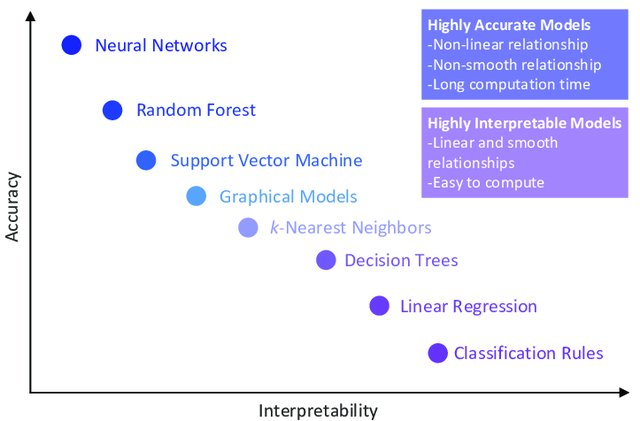
\includegraphics[scale=1.4]{images/interpretability_accuracy_tradeoff.jpg}
    \caption{The plot represented in this figure wants to highlight how different ML models are related to the trade-off between accuracy and intepretability \cite{morocho2019machine}. More a model is accurate such as Neural Network and Random Forest, more it's less interpretable due to its "black-box" nature.}
    \label{fig:trade-off}
\end{figure}
\subsection{Neural Network with Keras}
It's one of the deep learning algorithms which is based on the structure of biological neural network, where nodes represent neurons.
Nodes are connected to each others through the layers. 
In this way, every neuron of a layer is connected to neurons in the next layer.
The structure of my Neural Network is formed by 3 layers:
\begin{itemize}
    \item Input layer: Each node takes the initial data into the network and propagate information to the following layers;
    \item Output layer: It contains the result of the problem. 
    \item Hidden layer: It's actually responsible for performance and complexity of neural networks. It's placed between the output and input layers;
\end{itemize}
During the training phase, in which the network "learns", independent variables are used as input and processed through a weighted associations in which at each step produce a results which are compared to the target output. The error computed between them is successively adjusted and update following learning rules. The achievement obtained is a results increasingly similar to the values assumed by the target variable. 
For implementing it, I use Keras API from TensorFlow library.


\subsection{Machine Learning with Random Forest}
Random forests is used in regression problem, by using a structure of decision trees for making predictions. Decision trees answer to sequential questions through the routes tracked by trees.
Algorithm consists in building a certain number of random decision trees from the a bootstrap sample of the original data set (this phase is called bootstrap sampling). Then, the prediction of a certain sample is performed by following each decision trees. In a regression problem the final decision will be an averaged value from the ones obtained by each tree (phase of aggregation).
For implementing it, I use RandomForestRegressor class from sklearn library, configured with 300 random trees.
\bigbreak
In the next chapters each step will be described in depth about procedures adapted in the case of study and the results obtained.

\begin{figure}[H]
    \centering
    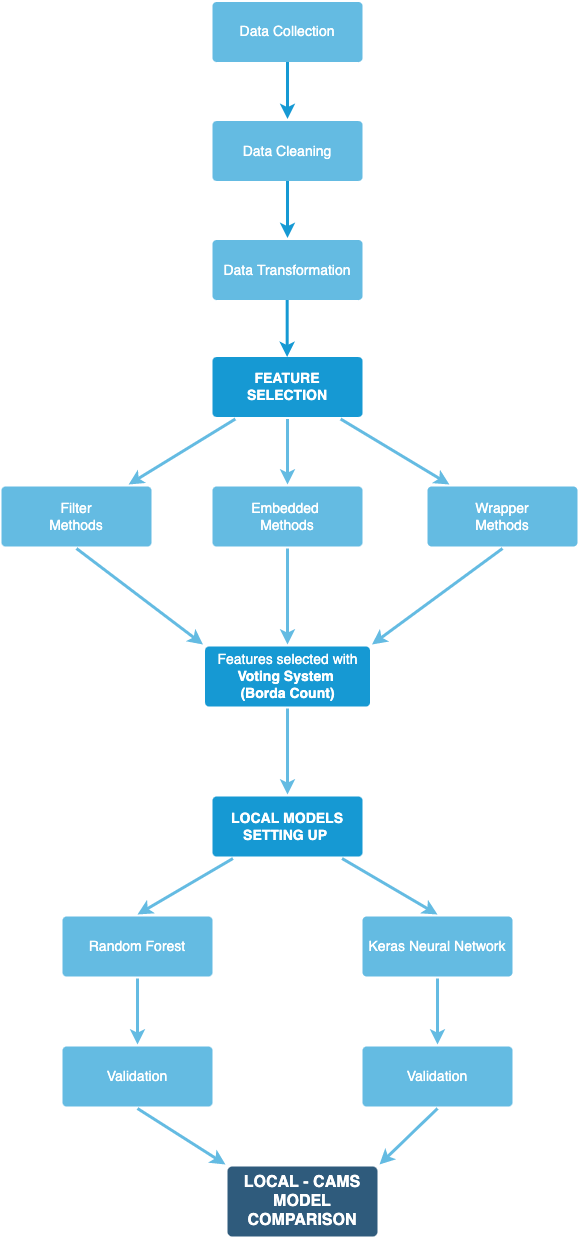
\includegraphics[scale=0.21]{images/overview.png}
    \caption{The following diagram give a general explanation of the procedure taken in this work thesis. It starts with the pre processing of the data (collection, cleaning and transformation) and continues with the selection of most meaningful variables (feature selection). \\
    After that, ML models are implemented and trained with the covariates chosen in the previous step. \\
    Finally an evaluation of the error metrics based on the validation is performed.}
    \label{fig:overview}
\end{figure}


\section{Notebook implemented}
For processing and analysing data I implemented tools collected in Python Notebooks, each one available in the D-DUST repository:
(\url{https://github.com/opengeolab/D-DUST/tree/thesis_MB}).\newline
Its essential steps are shown in figure \ref{fig:overview}.

\subsection{Computation and view of feature selection results}
In order to manage its configuration and the results obtained, a simple User Interface using ipywidgets package is built.
In this interface there are 2 sections:
\begin{itemize}
\item Feature Selection scores: they are graphically shown using multiple barplot, one for each data set previously selected. Barplot are implemented with the use of Plotly library; 
\item Options: in this box is possible to configure the feature selection input:
\begin{itemize}
\item target variable. Variable usable are the ones coming from ARPA ground sensors;
\item value of the Variance Threshold for discarding meaningless variable before FS (optional);
\end{itemize}
and the output:
\begin{itemize}
\item choice of method for visualize its own scores;
\item results normalization (optional);
\item order of the scores by descending order or by labels;
\item scale of Y-axis (regular or logarithmic);
\end{itemize}
\end{itemize}
A pseudo code of how the notebook works is atteched.
\begin{verbatim}
for each configuration in configurations
    for each period in periods
        #Data acquisition
        grid = input(period)
        grid = buffer_knn(grid)
        data_cleaning(grid)
        grid = VarianceThreshold(grid, 0.1)
        X, Y = get_variables(grid, target_variable)
        #Feature selection phase
        results = compute_feature_selection(X, Y)
    results = borda_count_algorithm(results)
    #results are stored externally in .csv files
    export_tocsv(results) 
    #results exported will have the feature ordered with respect
    #the score obtained with Borda Count algorithm
\end{verbatim}
\begin{figure}[H]
    \centering
    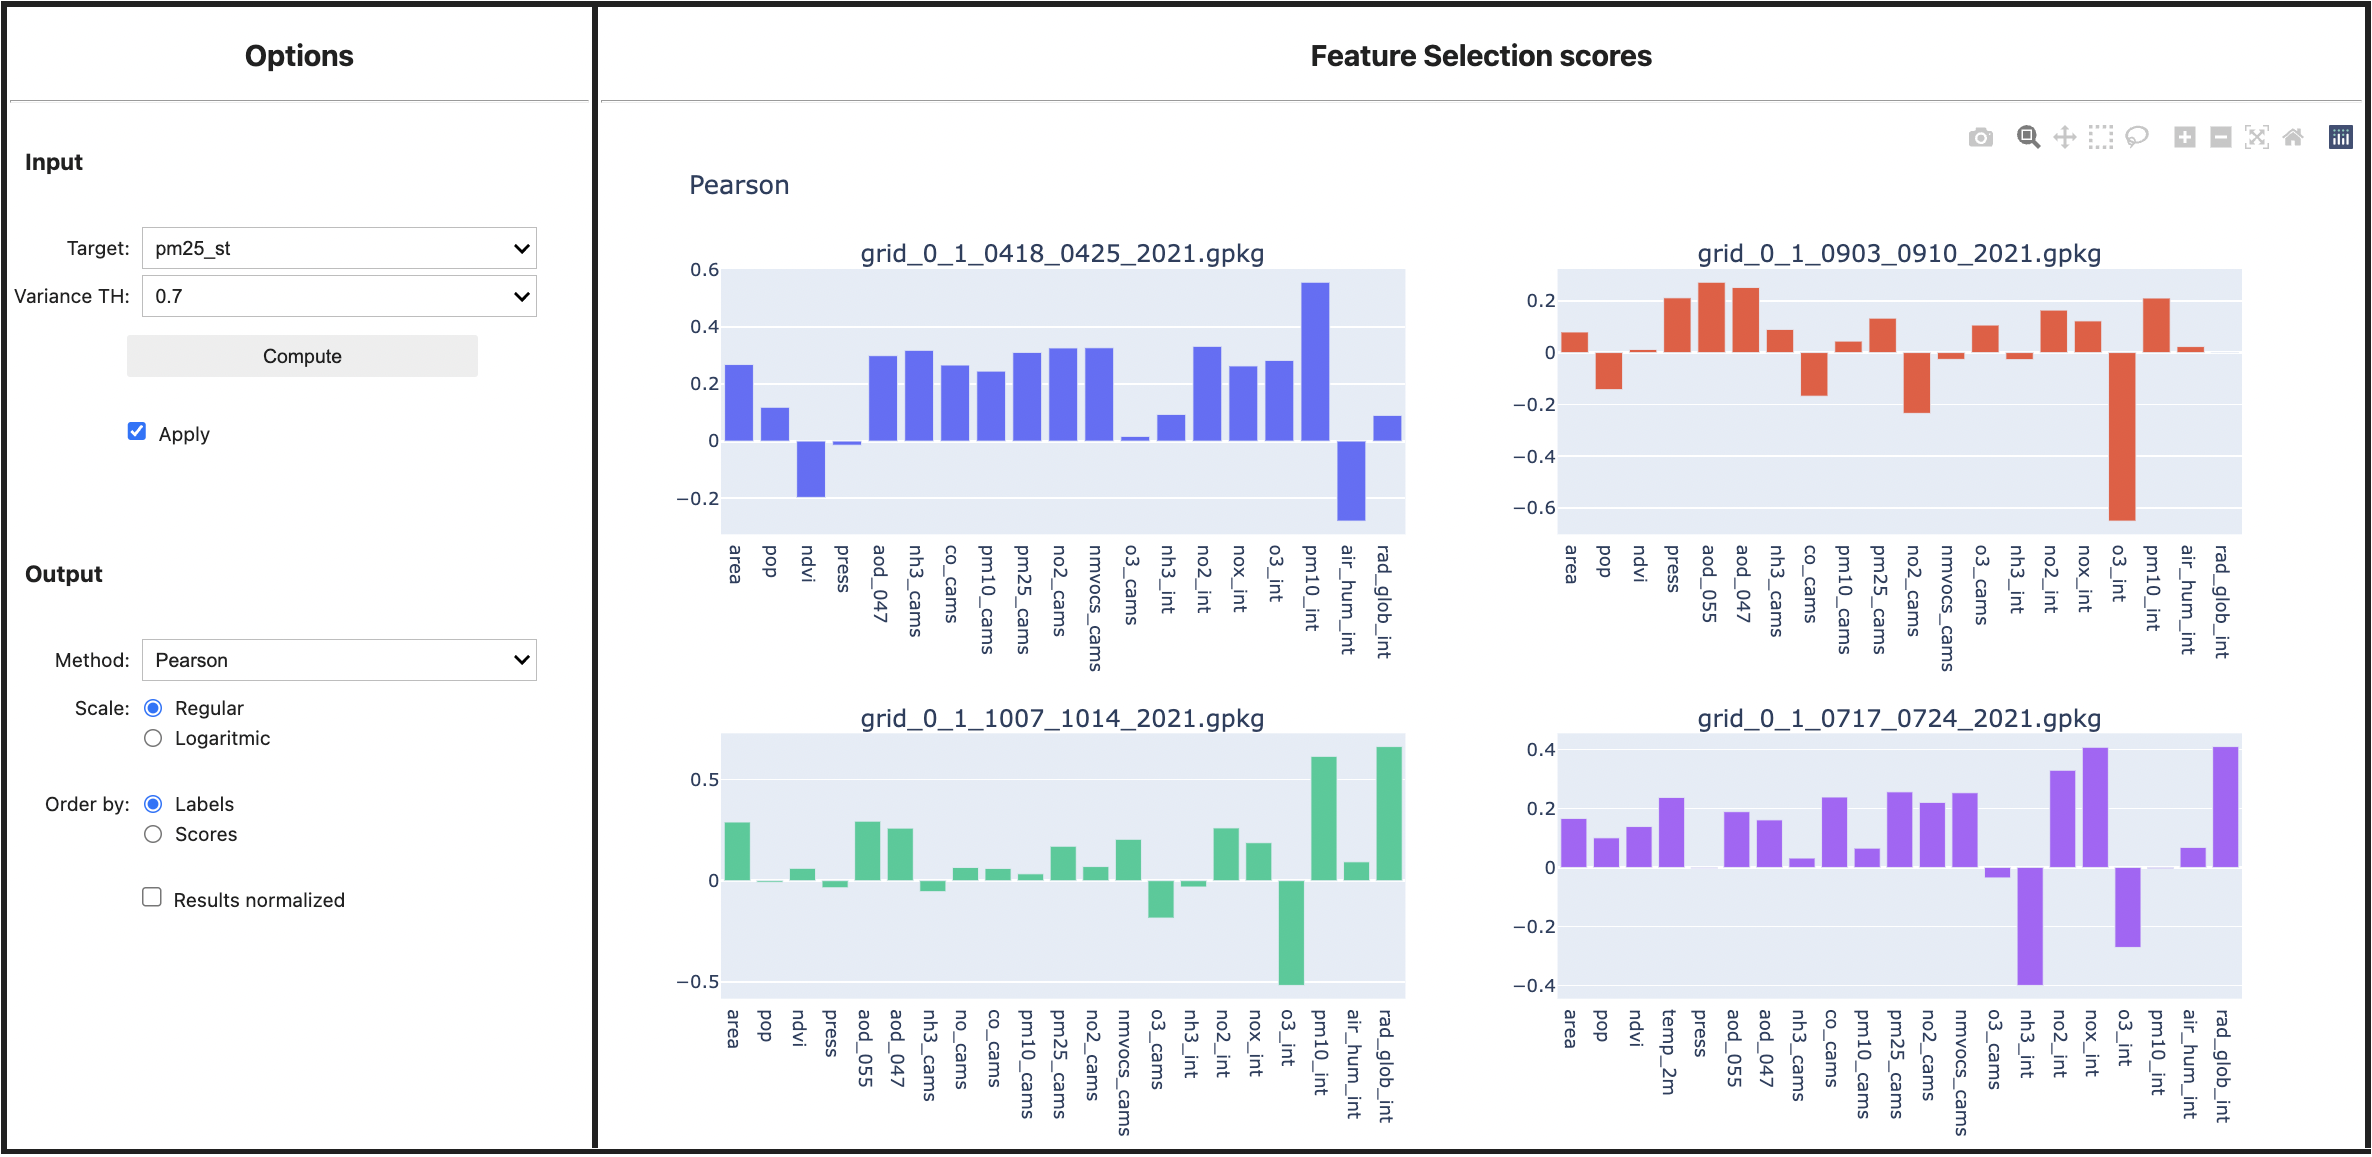
\includegraphics[scale=0.40]{images/notebook.png}
    \caption{Overview of the notebook implemented for FS procedure.}
    \label{fig:notebook}
\end{figure}

In the notebook are present also cells which aims to export FS results.

\subsection{Computation and view of ML models results}
For build I use 2 different notebook for the evaluation of the Neural Network (\href{https://github.com/opengeolab/D-DUST/blob/thesis_MB/notebooks/Keras_prediction_model.ipynb}{link}) and the Random Forest model (\href{https://github.com/opengeolab/D-DUST/blob/thesis_MB/notebooks/RandomForest_prediction_model.ipynb}{link}). 
It possible to set these parameter before running the model:
\begin{itemize}
    \item NUMBER\_OF\_COVARIATES: It's number of the n features with the highest Borda Count score take as input for the model;
    \item TARGET: It represents the target variable to be predicted by the model;
\end{itemize}
\begin{verbatim}
for each configuration in configurations
    results = []
    for each period in periods
        #Data acquisition
        grid = input(period)
        grid = buffer_knn(grid)
        data_cleaning(grid)
        X, Y = get_variables(grid, TARGET)
        X = get_n_columns(NUMBER_OF_COVARIATES)
        #Modelling in which training and validation is performed using k-fold
        model = new()
        model.training(X, Y)
        res = model.validation(X, Y)
        results.append(res)
    
    #results are stored externally in .csv files
    export(avg(results1))
    export(avg(results2))
 
\end{verbatim}

Each one of them imports the feature selected from the previous notebook and export the accuracy evaluation of the k-fold cross validation externally. \par
The results are subsequently opened and shown with \href{https://github.com/opengeolab/D-DUST/blob/thesis_MB/notebooks/model.ipynb}{this other notebook} through the use of widgets (\ref{fig:view}.
\begin{figure}[H] 
    \centering
    \subfloat[Drop-down widgets.]{%
        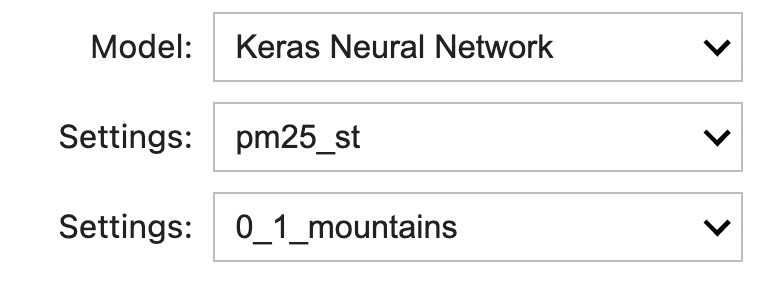
\includegraphics[width=0.5\textwidth]{images/dropdown.png}%
        %
        }%
    \hfill%
    \subfloat[Table with the results selected.]{%
        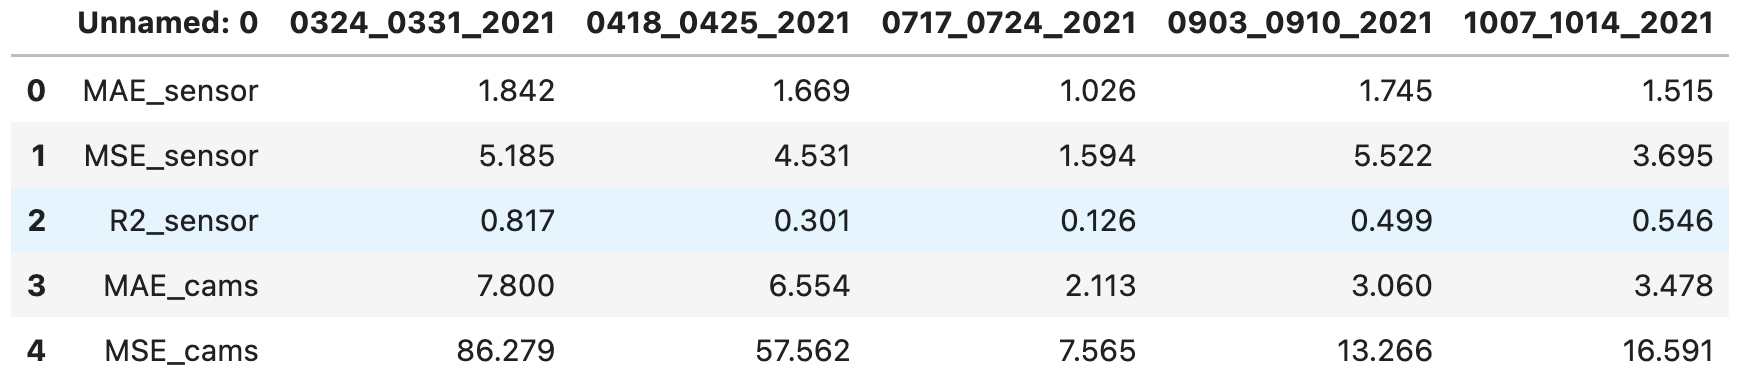
\includegraphics[width=0.5\textwidth]{images/table.png}%
        %
        }%
    \caption{In these images is illustrated how the notebook view for viewing the validation results works. It sufficient to select the target variable, resolution and configuration desired and with the an interactive option provided by ipywidgets library the results are provided through a table.}
    \label{fig:view}
\end{figure}

An overview of the order in which the different notebooks are used in my work thesis is illustrated in the figure .
\begin{figure}[H]
    \centering
    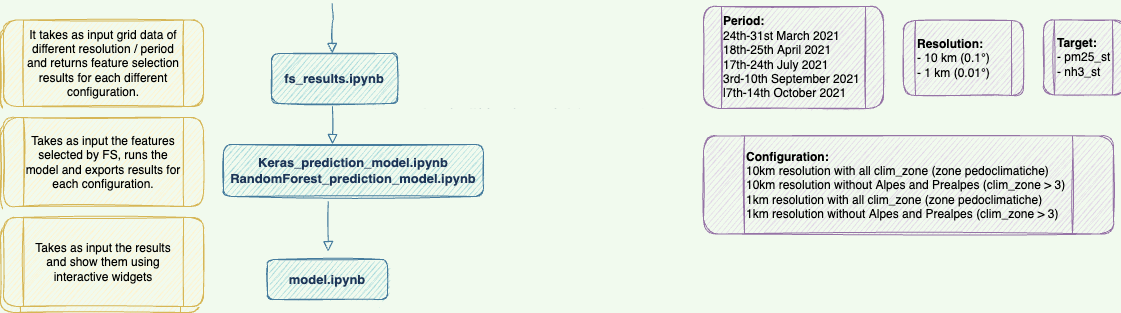
\includegraphics[scale=0.40]{images/overview _notebooks.png}
    \caption{The following diagram give a general explanation of the sequence of the notebooks which are used. It starts with fs\_results.ipynb which aims to collect, clean, transform and select the most meaningful variables through the Feature Selection). \\
    After that, Keras\_prediction\_model.ipynb and RandomForest\_prediction\_model.ipynb are used to implement ML models which are trained with the covariates chosen in the previous step. \\
    Finally the results of the error metrics based on the validation are provided by model.ipynb. 
    The results collected are each one configured with an initial VariancaThreshold method.}
    \label{fig:notebooks}
\end{figure} 

\chapter{Case of Study and Data Modelling }
 \label{chap:case}
In this chapter is explained the case of study inside the D-DUST project, paying attention on the data used in the different period, resolution and target variable. 

\section{Data sets description}
This case of study aims to discover the main factors which affects mostly the target variable chosen. 
Variables selected are the physical and chemical factors that are most associated with the formation of primary and secondary pollutant. \newline
Therefore, the variables are categorized in 4 different labels:
\begin{itemize}
\item Weather: These elements, such as wind speed and direction, precipitation and air temperature, changes in the epochs and can influence air pollution;
\item Pollutant: These variables represent primary and secondary pollutant related to the greenhouse effect;
\item Soil and Vegetation: Since soil and vegetation degradation are global concerns and can influence the air propagation in the environment, data related to local morphology are collected;
\item GIS (time invariant layers): This time-invariant layers are considered to be changeless in the time range considered. Differently from the other types which need a constant monitoring, these variables are update yearly with a lower frequency than the others;
\end{itemize}
Data chosen are open source and regularly available.
In this phase data have been collected (not by me but by other colleagues of D-DUST project at this \underline{ \href{https://docs.google.com/spreadsheets/d/1-5pwMSc1QlFyC8iIaA-l1fWhWtpqVio2/edit\#gid=91313358}{link}}) in grids from different sources and provided in geopackages. 
\subsection{Source types}
In order to better distinguish the data sources characteristics, variables selected are labelled with 4 different types of source:
\begin{itemize}

\item Ground Sensor: One of the aim of this case of study related to the D-DUST project, is to detect the impact on estimates combining data coming from ground sensor to satellites data, and analyse how the local monitoring could improve.  
Each ground monitoring stations which provide meteorological and air quality data belongs mainly to: 
\begin{itemize}
    \item ARPA (Agenzia Regionale per la Prevenzione dell'Ambiente);
    \item ESA Air Quality Platform (low cost sensor)\cite{esasensor};
\end{itemize}  
\item Model: data are estimated through a model built using satellite and meteorological and air quality data as input, such as European data provided by CAMS (Copernicus Atmosphere Monitoring Service);
\item Map layer: this data are time-invariant and are related to Lombardy morphology such as density of roads, population or land use; 
\item Satellite Sensor: They provide data from air quality observation mainly. Satellites provider are Sentinel-5P Tropomi and Terra \& Aqua MODIS;
\end{itemize}
\bigbreak

In the next lines each variable is provided in tables, by showing its type, name and description:

\subsection{Meteo Variable (Table)}
\begin{center}
\setlength{\arrayrulewidth}{1.5pt}

\begin{longtable}{ |p{2cm}|p{1.5cm}|p{2.3cm}|p{4cm}|p{1cm}|p{2cm}| } 
\hline
\textbf{Physical variable} & \textbf{Source type}  & \textbf{Variable name}  & \textbf{Description}  & \textbf{Unit}  & \textbf{Source}\\ 
\hline
\multirow{3}{4em}{Temperature} & Model  & \underline{temp\_2m} & Mean air temperature at 2 m above the land surface.\par & K & ERA5-Land hourly data.\\ 
& Ground \newline Sensor  & \underline{temp\_lcs} &  Mean air temperature ground measurement - Low Cost Sensor ESA monitoring stations.\par & °C & ESA Air Quality Platform.\\ 
& Ground \newline Sensor  & \underline{temp\_st} &  Mean temperature - ARPA monitoring stations.\par & °C & ARPA \newline Lombardia.\\ \hline
\pagebreak
\hline
\multirow{4}{4em}{Wind} & Model  & \underline{e\_wind} & Mean eastward wind component 10 m above the land surface.\par & m/s & ERA5-Land hourly data.\\ 
& Ground \newline Sensor  & \underline{n\_wind} &  Mean northward wind component 10 m above the land surface.\par & m/s & ERA5-Land hourly data.\\
& Ground \newline Sensor  & \underline{wind\_speed\_st} &  Mean wind speed on ground  - ARPA monitoring stations. \par& m/s& ARPA \newline Lombardia.\\ \hline

\multirow{2}{4em}{Precipitation} & Model  & \underline{prec} & Mean accumulated liquid and frozen water, including rain and snow, that falls to the Earth's surface. It is the sum of large-scale precipitation. \par & mm & ERA5-Land hourly data.\\ 
& Ground \newline Sensor  & \underline{prec\_st} &  Mean precipitation in each cell in the time range - ARPA monitor stations. \par & mm & ARPA \newline Lombardia.\\ \hline

\multirow{2}{4em}{Air Humidity} & Ground \newline Sensor  & \underline{air\_hum\_st} & Mean air moisture measurement in the time range - ARPA monitoring stations.\par & \% & ARPA \newline Lombardia.\\ 
& Ground \newline Sensor  & \underline{air\_hum\_lcs} &  Mean air moisture ground measurement - Low Cost Sensor ESA monitoring stations.\par & \% & ESA Air Quality Platform.\\ \hline

\multirow{1}{4em}{Air Pressure} & Model   & \underline{press} & Mean weight of all the air in a column vertically above the area of the Earth's surface represented at a fixed point.\par & Pa & ERA5-Land hourly data.\\ \hline

\multirow{1}{4em}{Solar Radiation} & Ground \newline Sensor  & \underline{press} & Global radiation measurement - ARPA monitoring station.\par & W/m\textsuperscript{2} & ARPA \newline Lombardia.\\ \hline

\hline
\caption{Table of Meteorological variables.}

\end{longtable}
\end{center}

\subsection{Pollutants Variables (Table)}


\begin{center}
\setlength{\arrayrulewidth}{1.5pt}
\begin{longtable}{ |p{2cm}|p{1.5cm}|p{2.3cm}|p{4cm}|p{1cm}|p{2cm}| } 
\hline
\textbf{Physical variable} & \textbf{Source type}  & \textbf{Variable name}  & \textbf{Description}  & \textbf{Unit}  & \textbf{Source}\\ 
\hline
\multirow{1}{4em}{Dust} & Model  & \underline{dust} & Mean dust concentration at 0m level provided by CAMS (Ensemble Median - Analysis).\par & ug/m\textsuperscript{3} & CAMS Model.\\ \hline

\multirow{3}{4em}{AOD} & Satellite \newline Sensor  & \underline{aod\_055} & Mean Aerosol Optical Depth at 550nm.\par & - & MODIS Terra+Aqua.\\ 
& Satellite \newline Sensor  & \underline{aod\_047} &  Mean Aerosol Optical Depth at 470nm.\par & - & MODIS Terra+Aqua.\\ 
& Satellite \newline Sensor & \underline{uvai} &  Mean UV Aerosol Index. A positive index highlights the presence of UV absorbing aerosol (such as smoke/dust). \par & - & Sentinel-5P\\ \hline

\multirow{3}{4em}{PM10} & Model  & \underline{pm10\_cams} & Mean PM10 concentration at 0m level provided by CAMS  (Ensemble Median - Analysis).\par & ug/m\textsuperscript{3} & CAMS Model.\\ 
& Ground \newline Sensor  & \underline{pm10\_lcs} &  Mean PM10 concentration ground measurement - Low Cost Sensor ESA monitoring stations.\par & not\newline defined & ESA Air Quality Platform.\\ 
& Ground \newline Sensor & \underline{pm10\_st} &  Mean PM10 concentration ground measurement - ARPA monitoring stations. \par & ug/m\textsuperscript{3} & ARPA \newline Lombardia\\ \hline

\multirow{3}{4em}{PM2.5} & Model  & \underline{pm25\_cams} & Mean PM2.5 concentration at 0m level provided by CAMS  (Ensemble Median - Analysis).\par & ug/m\textsuperscript{3} & CAMS Model.\\ 
& Ground \newline Sensor  & \underline{pm25\_lcs} &  Mean PM2.5 concentration ground measurement - Low Cost Sensor ESA monitoring stations.\par & ug/m\textsuperscript{3} & ESA Air Quality Platform.\\ 
& Ground \newline Sensor & \underline{pm25\_st} &  Mean PM2.5 concentration ground measurement - ARPA monitoring stations. \par & ug/m\textsuperscript{3} & ARPA \newline Lombardia\\ \hline
\pagebreak
\hline
\multirow{3}{4em}{SO\textsubscript{2}} & Model  & \underline{so2\_cams} & Mean SO\textsubscript{2} concentration at 0m level provided by CAMS  (Ensemble Median - Analysis).\par & ug/m\textsuperscript{3} & CAMS Model.\\ 
& Satellite \newline Sensor  & \underline{so2\_s5p} &  Mean SO2  vertical column density at ground level. \par& mol/m\textsuperscript{2} & Sentinel-5P.\\ 
& Ground \newline Sensor & \underline{so2\_st} &  Mean SO\textsubscript{2} concentration ground measurement - ARPA monitoring stations. \par & ug/m\textsuperscript{3} & ARPA \newline Lombardia.\\ \hline


\multirow{4}{4em}{NO\textsubscript{2}} & Model  & \underline{no2\_cams} & Mean NO\textsubscript{2} concentration at 0m level provided by CAMS  (Ensemble Median - Analysis).\par & ug/m\textsuperscript{3} & CAMS Model.\\ 
& Satellite \newline Sensor  & \underline{no2\_s5p} &  Mean NO2  vertical column density at ground level.\par & mol/m\textsuperscript{2} & Sentinel-5P.\\ 
& Ground \newline Sensor & \underline{no2\_st} &  Mean NO\textsubscript{2} concentration ground measurement - ARPA monitoring stations. \par & ug/m\textsuperscript{3} & ARPA \newline Lombardia.\\ 
& Ground \newline Sensor & \underline{no2\_lcs} &  Mean NO\textsubscript{2} concentration ground measurement - Low Cost Sensor ESA monitoring stations. \par & ug/m\textsuperscript{3} & ESA Air Quality Platform.\\ \hline

\multirow{1}{4em}{NO} & Model  & \underline{no2\_cams} & Mean NO concentration at 0m level provided by CAMS  (Ensemble Median - Analysis). \par& ug/m\textsuperscript{3} & CAMS Model.\\  \hline

\multirow{1}{4em}{CH\textsubscript{2}O} & Satellite \newline Sensor  & \underline{ch20\_s5p} & Mean Formaldehyde tropospheric column number density. \par& mol/m\textsuperscript{2} & Sentinel-5P.\\  \hline

\multirow{1}{4em}{CH\textsubscript{4}} & Satellite \newline Sensor  & \underline{ch20\_s5p} & Mean column averaged dry air mixing ratio of methane. \par& ppbV & Sentinel-5P.\\  \hline

\multirow{1}{4em}{NO\textsubscript{x}} & Ground \newline Sensor & \underline{nox\_st} &  Mean NO\textsubscript{x} (field: "Ossidi di Azoto") concentration ground measurement - ARPA monitoring stations.\par  & ug/m\textsuperscript{3} & ARPA \newline Lombardia.\\ \hline

\multirow{1}{4em}{CO\textsubscript{2}} & Ground \newline Sensor & \underline{co2\_lcs} &  Mean CO2 concentration ground measurement - Low Cost Sensor ESA monitoring stations. \par & ? & ESA Air Quality Platform.\\ \hline
\pagebreak
\hline
\multirow{4}{4em}{CO} & Model  & \underline{co\_cams} & Mean CO concentration at 0m level provided by CAMS  (Ensemble Median - Analysis).\par & ug/m\textsuperscript{3} & CAMS Model.\\ 
& Satellite \newline Sensor  & \underline{co\_s5p} &  Mean CO vertically integrated column density.\par & mol/m\textsuperscript{2} & Sentinel-5P.\\ 
& Ground \newline Sensor & \underline{co\_st} &  Mean CO concentration ground measurement - ARPA monitoring stations. \par & ug/m\textsuperscript{3} & ARPA \newline Lombardia.\\ 
& Ground \newline Sensor & \underline{co\_lcs} &  Mean CO concentration ground measurement - Low Cost Sensor ESA monitoring stations. \par & ug/m\textsuperscript{3} & ESA Air Quality Platform.\\ \hline

\multirow{3}{4em}{O\textsubscript{3}} & Model  & \underline{o3\_cams} & Mean O\textsubscript{3} concentration at 0m level provided by CAMS  (Ensemble Median - Analysis).\par & ug/m\textsuperscript{3} & CAMS Model.\\ 
& Satellite \newline Sensor  & \underline{03\_s5p} &  Mean O\textsubscript{3} total atmospheric column.\par  & mol/m\textsuperscript{2} & Sentinel-5P.\\ 
& Ground \newline Sensor & \underline{03\_st} &  Mean O\textsubscript{3} concentration ground measurement - ARPA monitoring stations.  \par& ug/m\textsuperscript{3} & ARPA \newline Lombardia.\\ 
 \hline
 
 \multirow{1}{4em}{CH\textsubscript{2}O}& Satellite \newline Sensor  & \underline{ch20\_s5p} &  Mean Formaldehyde tropospheric column number density. \par & mol/m\textsuperscript{2} & Sentinel-5P.\\ \hline
 
\multirow{1}{4em}{NMVOCs}& Model  & \underline{nmvocs\_cams} & Mean Non-Methane VOCs concentrations at 0m level provided by CAMS.\par & ug/m\textsuperscript{3} & CAMS Model.\\ \hline

\multirow{3}{4em}{NH\textsubscript{3}} & Model  & \underline{nh3\_cams} & Mean NH\textsubscript{3} concentration at 0m level provided by CAMS  (Ensemble Median - Analysis).\par & ug/m\textsuperscript{3} & CAMS Model.\\ 
& Satellite \newline Sensor  & \underline{nh3\_lcs} &  Mean NH\textsubscript{3} concentration ground measurement - Low Cost Sensor ESA monitoring stations. \par  & ? & ESA Air Quality Platform.\\ 
& Ground \newline Sensor & \underline{nh3\_st} &  Mean NH\textsubscript{3} concentration ground measurement - ARPA monitoring stations. \par & ug/m\textsuperscript{3} & ARPA \newline Lombardia.\\ \hline
\caption{Table of Pollutant variables.}
\end{longtable}
\end{center}
In addition to them, there's also pollutants variables ending with '\_int' (such as 'pm10\_int', 'pm25\_int', 'nh3\_int', etc.). These variables are obtained by interpolating ARPA variables which are not spatially continued. The explanation of how they are interpolated and how I mitigate the problem of having a limited number of observation from ground sensors along the surface is in one of the next \hyperref[subsec:nan]{subsection}.
\subsection{Soil and Vegetation (Table)}

\begin{center}
\setlength{\arrayrulewidth}{1.5pt}
\begin{longtable}{ |p{2cm}|p{1.5cm}|p{2.3cm}|p{4cm}|p{1cm}|p{2cm}| } 
\hline
\textbf{Physical variable} & \textbf{Source type}  & \textbf{Variable name}  & \textbf{Description}  & \textbf{Unit}  & \textbf{Source}\\ 
\hline

\multirow{3}{4em}{Vegetation} & Satellite \newline Sensor  & \underline{siarlX} & Fraction of area in each cell for each agricultural use provided by SIARL Catalog for Lombardy Region.\par & \% & SIARL Lombardia 2019.\\ 
& Satellite \newline Sensor  & \underline{ndvi} &  Mean NDVI cell value over 16 days period.\par & - & USGS Earth Data.\\ 
& Satellite \newline Sensor  & \underline{siarl} &  Majority class for agricultural use provided by SIARL Catalog for Lombardy Region. \par & cat & SIARL Lombardia 2019.\\
\hline

\multirow{5}{4em}{Soil} & Model  & \underline{soil\_moist} & Mean volume of water in soil layer 1 (0 - 7 cm) of the ECMWF Integrated Forecasting System. The surface is at 0 cm. The volumetric soil water is associated with the soil texture (or classification), soil depth, and the underlying groundwater level.\par & m\textsuperscript{3}/m\textsuperscript{3} & ERA5 Land Hourly Data.\\ 
& Map Layer  & \underline{soilX} &  Fraction of area for each cell containing the soil type obtained from OpenLandMap soil texture classification.\par & \% & OpenLandMap Soil Texture Class (USDA System).\\ 
& Map Layer  & \underline{soil\_textX} &  Mean NDVI cell value over 16 days period. \par & \% & Basi informative dei suoli - Geoportale Lombardia.\\ 
& Map Layer  & \underline{soil} &  Majority soil type for each pixel from OpenLandMap soil texture classification .\par & cat & OpenLandMap Soil Texture Class (USDA System) .\\ 
& Map Layer  & \underline{soil\_text} &  Majority soil type for each pixel from Carta pedologica 250K (Lombardy Region). \par& cat & Basi informative dei suoli - Geoportale Lombardia.\\ 

\hline
\caption{Table of variables referred to Vegetation and Soil.}

\end{longtable}
\end{center}

\subsection{GIS (static layers) (Table)}

\begin{center}
\setlength{\arrayrulewidth}{1.5pt}
\begin{longtable}{ |p{2.1cm}|p{1.5cm}|p{2.3cm}|p{4cm}|p{1.5cm}|p{2cm}| } 
\hline
\textbf{Physical variable} & \textbf{Source type}  & \textbf{Variable name}  & \textbf{Description}  & \textbf{Unit}  & \textbf{Source}\\ 
\hline
\multirow{1}{4em}{Geometry} & Map Layer  & \underline{area} & Area of Lombardy Region vector layer in each cell. \par& km\textsuperscript{2} & SIARL Lombardia 2019.\\ 
\hline
\multirow{1}{4em}{Calendar} & Map Layer  & \underline{cal} & JSON file containing the time-ranges used for data processing. \par& day & -\\ 
\hline

\multirow{1}{4em}{Population} & Map Layer  & \underline{pop} & Population for each cell. & n° of inhabitants& Gridded Population of the World (GPW).\\ \hline

\multirow{2}{4em}{Land use and cover} & Map Layer  & \underline{dsfX} & Land use fraction for each cell containing the classification the classification provided by DUSAF Catalog (Lombardy Region). & \% (fraction for each cell) & DUSAF Lombardia 2018.\\ \hline
Map Layer  & \underline{dusaf} & Cover & Land Use majority class for each cell provided by DUSAF Catalog (Lombardy Region). & cat  & DUSAF Lombardia 2018.\\
\hline

\multirow{3}{4em}{Terrain} & Map Layer  & \underline{h\_mean} & DTM average elevation for each pixel. & m & Geoportale Lombardia 2019.\\ 
& Map Layer  & \underline{aspect\_major} & Aspect derived from DTM. Majority pixel aspect. & Degree North & Geoportale Lombardia 2019.\\ 
& Map Layer  & \underline{slope\_mean} & Average slope derived from DTM. & Degree North & Geoportale Lombardia 2019.\\ 

\hline
\pagebreak
\hline
\multirow{6}{4em}{Road Infrastructures} & Map Layer  & \underline{int\_prim} & Density of intersection nodes between primary roads for each cell (including highways). & int\textsubscript{s}/km\textsuperscript{2} & Geoportale Lombardia 2019.\\ 
& Map Layer  & \underline{int\_prim\_sec} & Density of intersection nodes between primary and secondary roads for each cell. & int\textsubscript{s}/km\textsuperscript{2} & Geoportale Lombardia 2019.\\ 
& Map Layer  & \underline{int\_sec} & Density of intersection nodes between secondary roads for each cell. & int\textsubscript{s}/km\textsuperscript{2} & Geoportale Lombardia 2019.\\ 
& Map Layer  & \underline{prim\_road} & Density of primary importance roads for Lombardy Region inside for each. & km/km\textsuperscript{2} & Geoportale Lombardia 2019.\\ 
& Map Layer  & \underline{sec\_road} & Density of secondary importance roads for Lombardy Region foreach cell. & km/km\textsuperscript{2} & Geoportale Lombardia 2019.\\ 
& Map Layer  & \underline{highway} & Density of highways for Lombardy Region inside for cell divided. & km/km\textsuperscript{2} & Geoportale Lombardia 2019.\\ 
\hline

\multirow{1}{4em}{Farms building} & Map Layer  & \underline{farms} & Fraction of area covered by farms inside the cell. Obtained from DUSAF dataset. & \% (fraction for each cell) & DUSAF Lombardia 2018.\\ \hline
\multirow{1}{4em}{Breeding Farms} & Map Layer  & \underline{farm\_type} & Density of farms classified by breed type for each cell: poultry, pigs, sheeps. & farms/km\textsuperscript{2} & DUSAF Lombardia 2018.\\ \hline
\multirow{1}{4em}{Air quality zones} & Map Layer  & \underline{aq\_zone} & Majority class of a given air quality zone in each cell. & cat  & Geoportale Lombardia.\\ \hline
\multirow{1}{4em}{Climate zones} & Map Layer  & \underline{clim\_zone} & Majority class of a given air quality zone in each cell. & cat  & - \\ \hline


\hline
\caption{Table of Static GIS variables.}

\end{longtable}
\end{center}
\pagebreak

\subsection{Categorical Variables (table)}
Categorical data are identified with names or labels given to them as value. Even if are represented by numbers, they don't have the same mathematical meaning as a numerical value. This type of data is discarded during the pre processing phase, since feature selection is done exclusively on numerical input and output values. 
In the following table is explained the semantic of the values assumed.
\bigbreak
\begin{center} 
\setlength{\arrayrulewidth}{1.5pt}
\begin{longtable}{ |p{2.5cm}|p{10cm}| } 
\hline
\textbf{Variable name} & \textbf{Note}\\ 
\hline

 \multicolumn{2}{|c|}{\textbf{Meteo}} \\
\hline
 \underline{wind\_dir\_st}  \newline \newline (Wind direction from ground sensor divided in 8 sectors). & 1 = North: 0° - 22.5° / 337.5° - 360°; \newline2 = North-East: 22.5° - 67.5°; \newline3 = East: 67.5° - 112.5°;  \newline4 = South-East: 112.5° - 157.5°; \newline5 = South: 157.5° - 202.5°; \newline6 = South-West: 202.5° - 247.5°; \newline7 = West: 247.5° - 292.5°; 8 = North-West: 292.5° - 337.5°\\ \hline
 \multicolumn{2}{|c|}{\textbf{Soil and Vegetation}} \\ \hline
 \underline{siarl} \newline \newline (Majority class for agricultural use provided by SIARL Catalog for Lombardy Region). & 2 = Cereal; \newline9 = Mais; \newline12 = Rice;\\  \hline
 \underline{soil} \newline \newline (Majority soil type for each pixel from OpenLandMap soil texture classification). &  1 = Clay; \newline2 = Silty Clay; \newline3 = Sandy Clay; \newline4 = Clay Loeam; \newline5 = Silty Clay Loam; \newline6 = Sandy Clay Loam; \newline7 = Loam;\newline8 = Silt Loam; \newline9 = Sandy Loam; \newline10 = Silt; \newline11 = Loamy Sand; \newline12 = Sand;  \\ \hline 
\underline{soil\_text} \newline \newline (Majority soil type for each pixel from Carta pedologica 250K). & 1 = Fine clay;\newline 2 = Very fine clay;\newline  3 = Fine loose;\newline  4 = Coarse loose;\newline  5 = Fine silty;\newline  6 = Coarse silty;\newline  7 = Skeletal-clayey sand;\newline  9 = Skeletal-loose;\newline  10 = skeletal-sand; \\ \hline
 \multicolumn{2}{|c|}{\textbf{GIS (Static layers)}} \\ \hline
 \underline{dusaf} \newline \newline (Land use and cover). & 2 = Agricultural areas; \newline3 = Wooded territories and semi-natural environments; \newline4 = Wetlands; \newline5 = Water bodies; \newline11 = Urbanised areas; \newline12 = Production facilities, large plants and communication networks; \newline13 = Mining areas, landfills, construction sites, waste and abandoned land; \newline14 = Non-agricultural green areas; \\
\hline
 \underline{aq\_zone}\newline \newline (Air quality zones) & 1 = Highly urbanized plains; \newline 2 = Plains; \newline 3 = Prealpi, Appennino and mountains;\newline 4 = Valley floor Agg; 
\newline5 = Urban agglomarated area (Milano, Bergamo, Brescia);\\
\hline
 \underline{clim\_zone}\newline \newline (Climate zones) & 1 = Alpi;\newline 2 = Prealpi Occidentali; \newline 3 = Prealpi Orientali;\newline 4 = Pianura Occidentale;\newline 5 =  Pianura Centrale;\newline 6 = Pianura Orientale; 
 \\
\hline
\caption{Table of categorical variables with their values legend.}



\end{longtable}
\end{center}
\pagebreak

In order to examine the behavior of each variable in a data set over time, several grid data are collected, each one with different resolution, period and configuration.
\subsection{Spatial resolution}
Vector grids that are used in the D-DUST project are three and they are generated by the spatial resolution of the source provider. 

\begin{itemize}
\item Grids with with Copernicus CAMS resolution (0.1°); resolution with Copernicus CAMS (European);
\item Grids with 0.01° Grid defined with maximum one ARPA station for each cell;
\end{itemize}

Data are scaled and fit in each spatial resolution grid in order to better analyse the final output model by considering each of them. 

\par
\subsection{Period}  
Data collected are dated 2021 because are the most recent and, with respect 2020, the ones not particularly affecting by emission reduction caused by lockdown for COVID-19 pandemic\cite{bontempi2022analysis}. 

In this case of study grid data are chosen by considering the effect of intensive agriculture, with these particular condition:
    \begin{itemize}
        \item In order to have right condition for farming, in the period chosen the terrain shouldn't be frozen (Temperature > 0°C). So I selected data coming from spring, summer and autumn period (discarding winter);
        \item For better highlighting the effect of intense agriculture with the usage of fertilizer and pesticides, which are the main pollution emission factors, weeks with no precipitations are selected;
\end{itemize}
In this way, several grid data are chosen from 5 different weeks:
\begin{itemize}
    \item 24 March - 31 March 2021;
    \item 18 April - 25 April 2021;
    \item 17 July - 24 July 2021;
    \item 3 September - 10 September 2021;
    \item 7 October - 14 October 2021
\end{itemize}

\subsection{Target Variables}
In this study target variables chosen represent the pollution phenomena correlated to agriculture intensive  such as the PM25 and Ammonia emissions. We choose these targets because are the most relevant sources of pollution produced by them.\newline
One of the aim of this step is to detect main pollutant factors which contribute further on the training of PM25 or NH3 emissions.
PM25 and ammonia (NH3) provided by ARPA sensors are the ones chosen as target variables('pm25\_st' and 'nh3\_st').
I choose measurement from ground sensor because are direct observation, more precises with the aim to support in this case of study local air quality monitoring. 
ARPA air quality monitoring stations, which, operating 24 h a day 365 days a year, are periodically checked and subject to maintenance, for ensuring the proper functioning and reliability.

\subsection{Mountains}
Another important parameter configuration used is to filter or not the cell covered by mountains or not (climate zone = 1/2/3 of Alpes and Prealpes). In this way the test run can take in consideration or not only urban and land areas, which are more affected by air pollution phenomena.

Firstly data covariates are divided between input (X) and output variable (Y). X represents all of variables collected in the previous part, excepting for the pollutant to be analysed and modelled (such as PM25 or Ammonia) which is assigned to the Y variable.


\section{Data Cleaning of NaN and low-variance values }
\label{subsec:nan}
In my work I consider as target variable PM25 and Ammonia coming from ground sensor measurement.
Air quality monitoring is usually carried out through ground sensors networks, which represents the primary air quality data source by governance. \newline
In the grids processed there's the problem that a given value provided by measurement tools (such as ground and satellite sensor) could be NaN. 
It's feasible since:
\begin{itemize}
\item A sensor could have no measurement for a given time epoch;
\item The set of sensor, because of its limited supply, cannot cover each cell of a grid;
\end{itemize}
In our case variable provided by ARPA and ESA ground sensor (with the label that ends with '\_st' and '\_lcs' respectively) has many NaN cells.
\par
However, no country in the world has yet established a monitoring network with a full satisfying coverage\cite{liu2018improve}. Even in the United States (US), which is characterized by a relatively developed PM2.5 ground monitoring network with 2500 stations has many areas unmonitored\cite{liu2018improve}. \par
Due to the fact that with data cleaning it results a data set with a very limited number of sample \cite{zhang2018strategy}, I perform previously a k-nearest neighbour classifier\cite{taunk2019brief} for detecting the buffer of cells closed to the location of the ground stations measurement. For increasing the number of observation provided by the limited ARPA stations in Lombardy a k-nearest neighbors algorithm is applied to adding the buffer of values (with k respectively equal to 10 for 0.1° and 30 for 0.01° resolution).  
Then, these cells are set with values computed using a Radial Basis function interpolation\cite{wright2003radial} which are separately stored in variables with name that ends with '\_int'. The given procedure available on GitHub \newline
In this way the size of the final sample, as the performance of the feature selection, would increase.
\par
Before the feature selection phase, VarianceThreshold was applied in order to discard variables with variance less than 0.1. 
\begin{figure}[H] \centering
{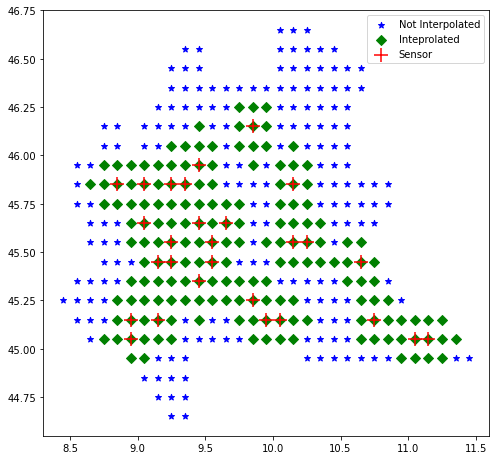
\includegraphics[scale=0.45]{images/buffer.png}}
 { \caption{Graphical representation of how buffer values interpolated from PM2.5 sensors provided by ARPA are added through k-nearest neighbour.}}
\end{figure}
\section{Feature Selection}
In this phase, I got the list of the most significant variables for each different configuration.
For doing that, after the features are selected for each period, an average of them is performed using again Borda Count algorithm. What is obtained is a general set of variables for each different configuration.
This was computed by averaging the feature selected for each different period with Borda Count another time;
Since I assume 2 different resolution and with the possibility to include or not the mountain zones, I obtained 4 different configurations: 
\begin{table}[H]
    \centering
    \begin{tabular}{|l|}
    \hline
        10km resolution (0.1°) with all clim\_zone (zone pedoclimatiche)  \\ \hline
        10km resolution (0.1°) without Alpes and Prealpes (clim\_zone > 3) \\ \hline
        1km resolution (0.01°) with all clim\_zone (zone pedoclimatiche)   \\ \hline
        1km resolution (0.01°) without Alpes and Prealpes (clim\_zone > 3)  \\ \hline
 
    \end{tabular}
\end{table}
In the \ref{fig:test_params} is shown a summary of the parameter of each test execution.
It can be observed that for each parameter there are different configurations: there are 2 resolutions, 2 climate zones parameter and 5 periods. Thus, for each different target variable, have been run 2x2x5 = 20 different tests both for ammonia and fine particulate (40 in total). 
Results from different periods for simplicity are grouped and averaged. In total in this work are attached 8 different results. Each results will be in detail pointed in the final Appendix TODO.
\begin{figure}[H]
    \centering
    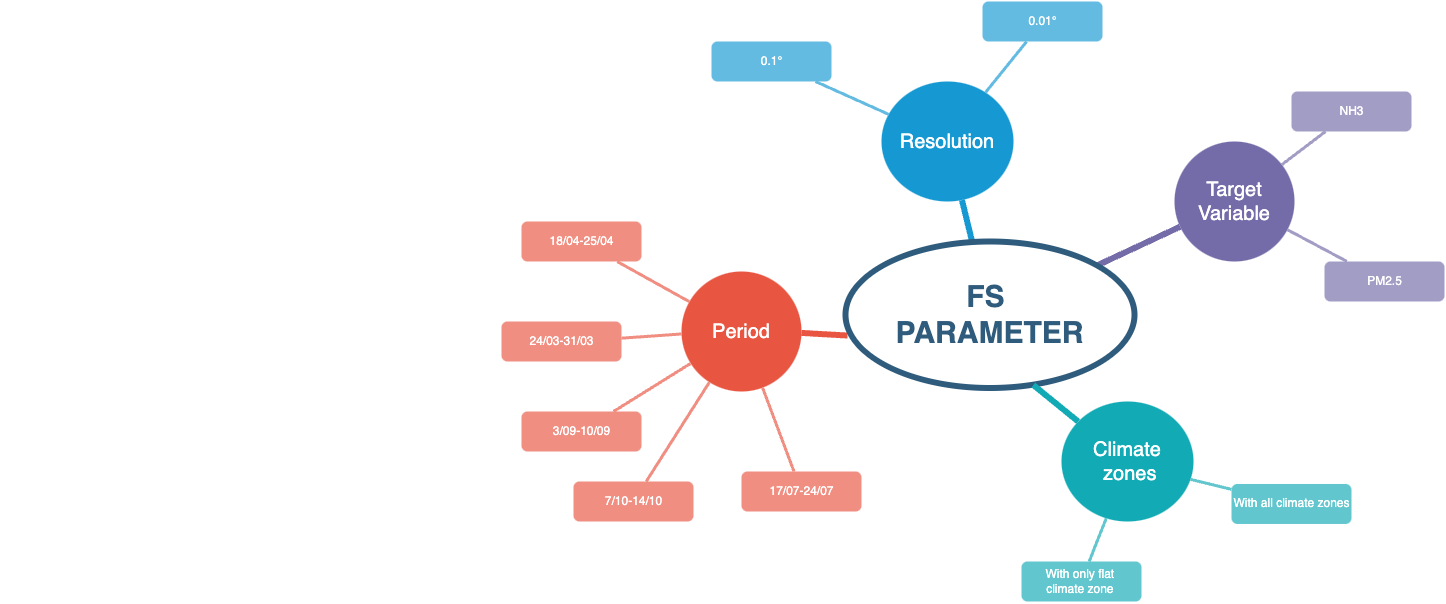
\includegraphics[width=.9\textwidth]{images/test_param.png}
    \caption{Parameter taken in consideration for tests execution.}
    \label{fig:test_params}
\end{figure}


\section{Data Modelling}
In this phase I evaluate models trained by variable selected by FS in order to analyze their interpretability and performance.
In detail the test run are built and validated using a k-fold (with k = 5) cross validation for mitigating undesirable over-fitting. 
I perform tests in 2 different ways, explained in the next subsections.
\subsection{Test for each period with CAMS comparison}
The validation made on the model was performed with 2 different variables values. They've been chosen:
\begin{itemize}
\item values of the target variable (ARPA measurements);
\item values assumed by the CAMS model;
\end{itemize}
Such a procedure was applied both to evaluate performance of the current model and to compare it to the CAMS model.
In this way, a comparison between results from these 2 different validations is performed, aiming to detect how much the models perform better in this local scale.\par
This is was applied for each data set obtained by the combinations of 4 configurations, 5 periods and 2 target variables (4x5x2 = 40 different model testes). 
\subsection{Test for analyse FS impact on performance}
In order to evaluate how Feature Selection affect positively the accuracy of the model a set of tests are run and configured differently from the previous. 
Data of different periods were merged together in order to develop the model through a temporal analysis, where the data are used in this way:
\begin{itemize}
    \item grid data from March, April and July periods were used from training;
    \item grid data from September and October were used for validation;
\end{itemize}

Totally were performed 8 tests, for each configuration and target variable (4 configuration x 2 target variables = 8)

https://www.sciencedirect.com/topics/agricultural-and-biological-sciences/agricultural-pollution 
https://pure.iiasa.ac.at/id/eprint/14769/1/Reduction%20of%20NH3%20emissions%20from%20agriculture%20in%20the%20Hai%20River%20Basin%20in%20China.pdf

https://towardsdatascience.com/batch-mini-batch-stochastic-gradient-descent-7a62ecba642a

\chapter{Results and Interpretations }
 \label{chap:res}
In this chapter are collected interpretations of the results obtained in the Feature Selection and the models' performance. All other tests not included in this chapter are available in the appendix \ref{chap:appendix}.
\\
\section{Feature Selection Results}
In this section the results obtained for each target variable selected are explained in relation to the:
\begin{itemize}
    \item votes received through Borda Count algorithm;
    \item positive or negative correlation assumed in the filter methods;
    \item confirmation in literature where a given correlation occurred; 
\end{itemize}
Similarities between the tests run for each target variable are visible for many factors that influence both particulate matter and ammonia.\\
This can be observed by the similarity of both positive and negative correlation from indexes from filter methods. \\
In the figure \ref{fig:pearson_general} are shown the results of the Pearson index, a filter method used during the FS. 
\begin{figure}[H]
\centering
\subfloat[pm25\_st as target variable.]{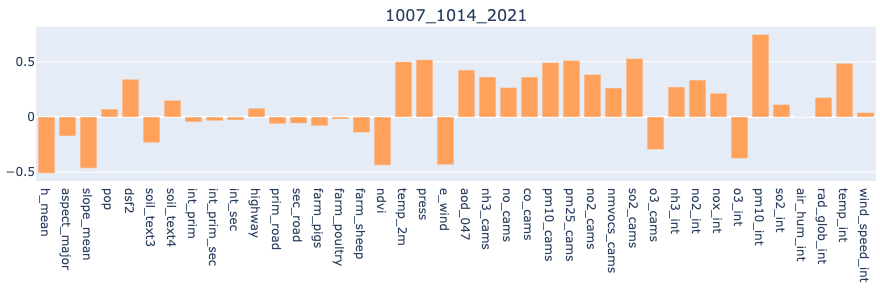
\includegraphics[scale =0.45]{images/tests/pm25pearson_october_0_01_mountains.png}}\\
\subfloat[nh3\_st as target variable.]{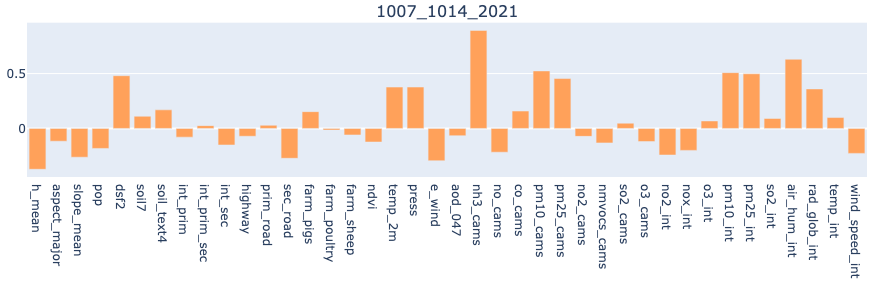
\includegraphics[scale =0.45]{images/tests/nh3_pearson_october_0_01_mountains.png}}
\caption{Pearson index results obtained in the period between 7-14 October with 1km resolution including mountains.}
\label{fig:pearson_general}
\end{figure}
The two bar plots attached aims to compare the scores obtained in the same period by the 2 target variables chosen in my tests in the October period.
One similarity between them is the influence of meteorological and morphological parameters.
By figure it appears that DTM average elevation and slope ('h\_mean' and 'slope\_mean' respectively) are correlated in the same way in the test of both target variables, since air pollution affects more urban than mountain areas.\\
Pollutants are negatively correlated to wind speed ('e\_wind'), since their concentration tends to turn down with it.\\ 
Indeed, the wind is a marker for the horizontal transport of air pollutants. Pressure also contributes to them ('press'), since it causes stable atmospheric conditions that make pollutants harder to be disseminated.
\par
In the test run the findings didn't  consistent differences if Alpes and Prealpes zones are included or not.\\
The only slight diversity found is about the votes obtained by pollutant and vegetation variables, which tend to be generally higher if mountain zones are excluded.
\subsection{PM2.5 as target variable}
Fine particulate matter (PM2.5) is one of the most common air pollutants in our environment. 
It comes primarily from transport vehicles (such as cars, trucks and buses), industry, burning of fuels and household activities. \\
During the 5 periods, it has been shown that PM2.5, as the other pollutants, changes over time. Air pollution changes accordingly to the type of climate and atmospheric conditions.\\
Below are atteched the table \ref{tab:statspm25} and the figure \ref{fig:graphstatspm2.5} that show PM2.5 variation in the 5 periods chosen in this case study.
\begin{table}[H]
\centering
\begin{tabular}{lrrrrr}
\toprule
 Statistic &  24/03-31/03 &  18/04-25/04 &  17/07-24/07 &  3/09-10/09 &  7/10-14/10 \\
\midrule
  Mean  &        30.217  &         18.203  &         12.974 &       15.450 &       14.878 \\
Median  &        27.938 &        17.938 &        13.063 &       14.75 &       15.281 \\
 Standard deviation &        3.772 &        3.462 &        1.831 &       4.000 &       3.166 \\
  Min value &        20.0  &        11.875 &        9.5 &        8.625 &       9.0 \\
  Max value &        42.0 &        25.714 &        17.375 &        27.875 &       19.625 \\
\bottomrule
\end{tabular}
\caption{Summmary statistics (measured in $\mu$g/m\textsuperscript{3}) of the PM2.5 provided by ARPA with 10 km resolution.}
\label{tab:statspm25}
\end{table}
\begin{figure}[H]
    \centering
    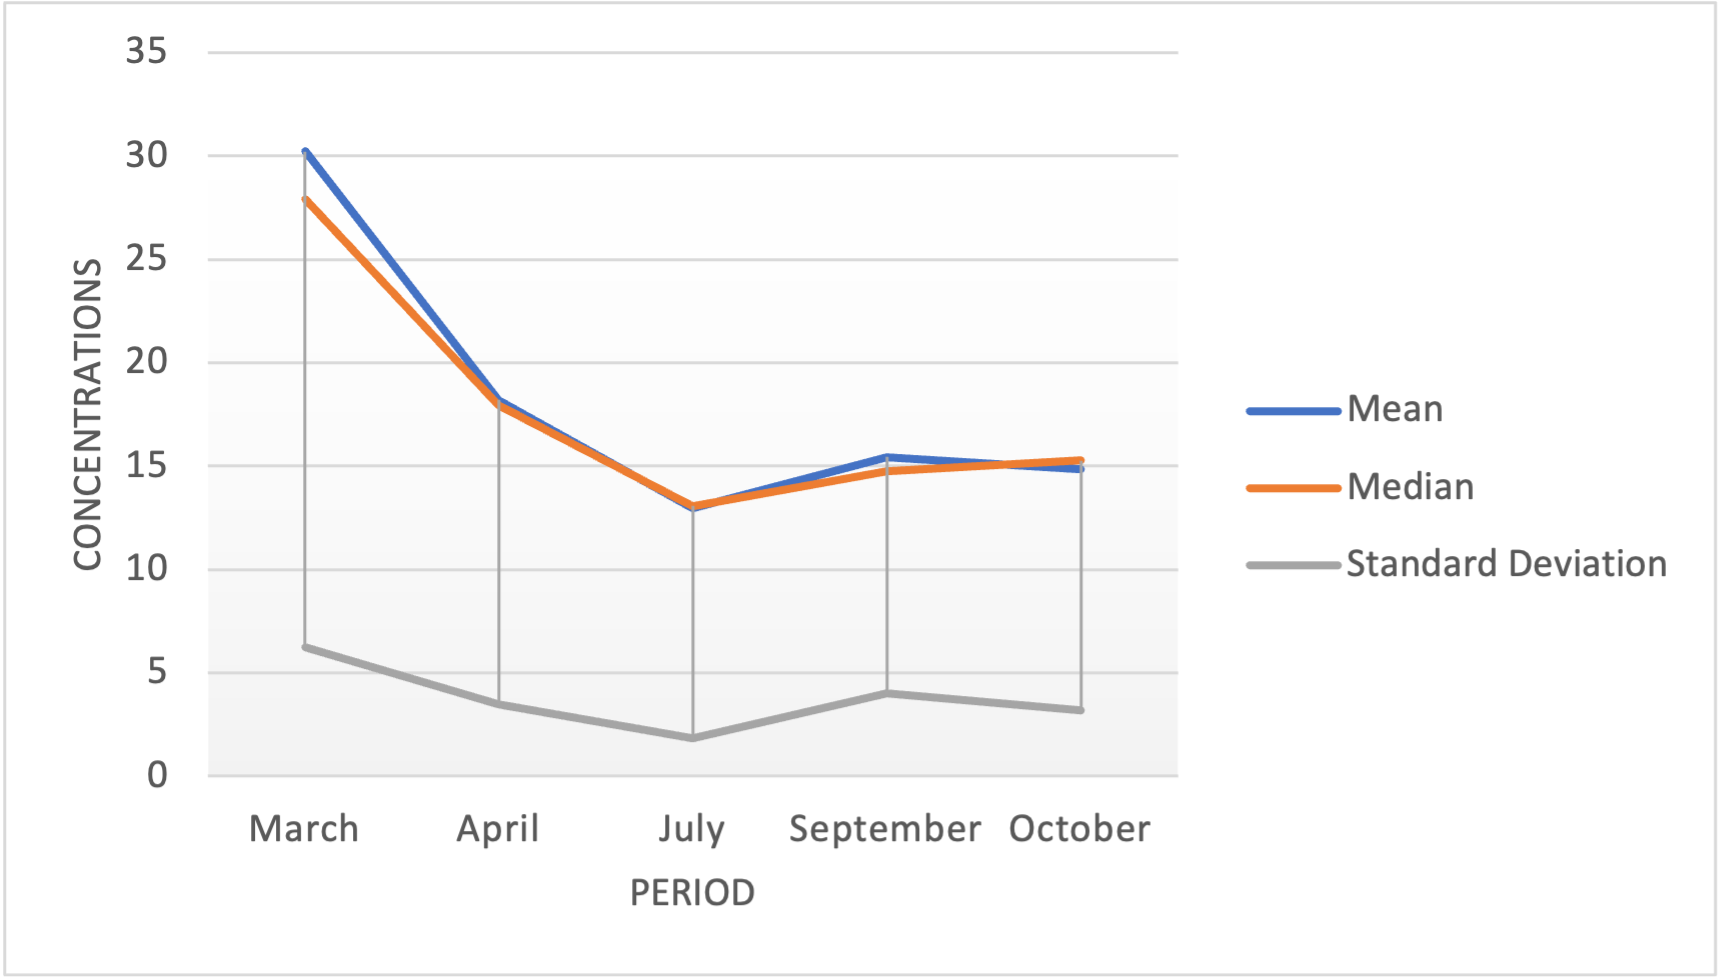
\includegraphics[scale=0.8]{images/pm25_values.png}
    \caption{Graphical representation of PM2.5 variation over the 5 periods, in relation of its mean, median and standard deviation (measured in $\mu$g/m\textsuperscript{3}).}
    \label{fig:graphstatspm2.5}
\end{figure}
In this subsection I comment the results obtained by FS of the figure \ref{fig:a}.
Air pollution analysis can confirm the presence of a high amount in the winter and heating season and a low quantity in the summer months \cite{cichowicz2017dispersion}. This is not applied to the ozone ('o3\_int' and 'o3\_cams'), which should be, on the contrary, higher during summer due to a combination of heat and sunlight which reacts with nitrogen oxides (NOx) and volatile organic compounds.\\
Indeed, ozone receives in the results many votes for its negative correlation (the highest in summer period), because is inversely related to PM2.5.\\
By the bar plots attached in the figure \ref{fig:fs_pm25}, it is clear that most of the pollutants have a strong or moderate correlation with PM2.5. \\
In particular, PM10 provided by ARPA and CAMS, in the various test executed is one of the most correlated pollutants. Indeed, 'pm10\_int' and 'pm10\_cams' have always a high number of votes.
A strong positive correlation between PM2.5 and PM10 is also demonstrated in the literature \cite{zhou2016concentrations}.
Another variable which received a strong number of votes is the PM2.5 modelled by CAMS ('pm25\_cams'). \\
Both variables, in fact, measure the same pollution phenomena.
This finding makes us understand how both variables are correlated even if measuraments were performed in 2 different way. PM2.5 from ARPA consists in measurament provided by fixed-ground sensor.\\
Instead, the PM2.5 from CAMS is provided by a global monitoring model, resulting from an ensemble median analysis of other models.
Indeed, the correlation coefficient between them is close to 1 in all tests executed.\\
It is visible a correlation with nitrogen dioxide('no2\_int'), a strong greenhouse gas which is related, as particulate matter, to biomass burning, industrial processes, households and road transport \cite{zellner2000john} \cite{maranzano2022air}.\\
There is also clear correlation with nitrogen oxides ('nox\_int'), nitrogen monoxide ('no\_int') and carbon monoxide ('co\_int', 'co\_cams, 'co\_s5p'). This could be explained by the fact that this pollutants contribute as a secondary pollutant to PM2.5 formation \cite{xie2015spatiotemporal}.
\par
Observing the results regarding intensive farming activities , it is evident that ammonia ('nh3\_int' and 'nh3\_cams') received, as PM10, most votes of all in the spring period due to its strong positive correlation (it can be observed in the figure \ref{fig:b}). \\
This happens because NH3 can react in the atmosphere to form ammonium salts in the presence of acid species \cite{viatte2021ammonia}.\\
We can assume that the main source of ammonia emission is intensive farming activities  since it was responsible for 92\% of the total by EEA country members in 2017 \cite{maranzano2022air}.\\
Indeed, during these periods, the application of fertilizer contributes to ammonia and particulate matter.\\
Significantly more fertilizer is applied in the spring than in the summer and winter seasons due to crop cycles \cite{goebes2003ammonia}.\\
Therefore, we can assume that intensive farming activities  is one of the factors that influence the formation of PM2.5, with the greatest contribution during a certain period of the year.
\begin{figure}[H]
\centering
\subfloat[Borda Count algorithm results.]{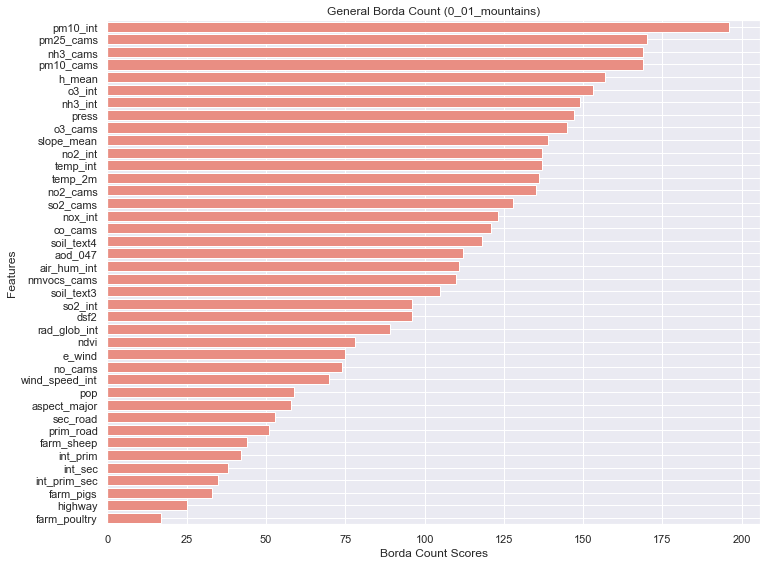
\includegraphics[scale =0.45]{images/tests/0_01_mountainspm25_st.png}\label{fig:a}}\\
\subfloat[Pearson index results in the  24-31 March and 18-25 April periods.]{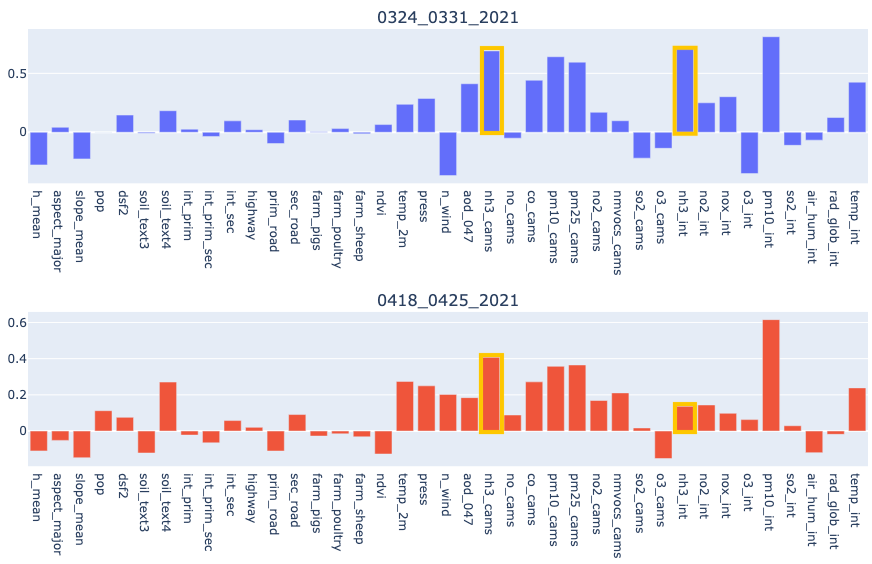
\includegraphics[scale =0.40]{images/tests/ammonia_effect_on_pm25_001mountains.png}\label{fig:b}}
\caption{Results obtained assuming PM2.5 as target variable with 10 Km resolution including mountains.}
\label{fig:fs_pm25}
\end{figure}
\subsection{NH3 as target variable}
Ammonia (NH3) is a reactive and soluble alkaline gas. It is one of the main sources of nitrogen pollution and comes from natural and anthropogenic sources, such as agriculture.\\
The process of ammonia evaporation commonly takes place when nitrogen is originated by the urea of animal livestock, and fertilize. \\
In the results obtained along the five periods, the ammonia provided by the CAMS model ('nh3\_cams') stands out, because it is strongly correlated, and represents the same pollutant as well.
We can observe in figure \ref{fig:fs_nh3} also variable related to PM10 and PM2.5 ('pm10\_int', 'pm10\_cams', 'pm25\_int' and 'pm25\_cams'), because ammonia contribute for the formation of secondary particulate matter \cite{dai2019concentrations} \cite{zhu2015sources}.\\
Correlation of ammonia in relation to intensive agriculture should be visible by the high positive correlation with agricultural areas (modelled by 'dsf2' variable), in particular used for maize cultivation ('siarl9') .\\
It is observable also the votes received by the variable that models the soil moisture, always with a positive correlation in relation to the target variable. This could be explained by the abundance of ammonia-oxidizing bacteria that increase with soil moisture \cite{avrahami2007response}.  \\
Other important weighted features are the ones related to intense farming ('farms' and 'farm\_pigs') which are responsible for ammonia release thanks to the chemical reaction of urea.\\
In fact, animal urine and faeces imply the release of ammonia and methane in the atmosphere, respectively \cite{saggar2004review}.
So we can suggest that ammonia in Lombardy should be very related to the use of fertilizer in agricultural areas and animal livestock in farms.
\bigbreak
\pagebreak
\clearpage
\begin{figure}[H]
\centering
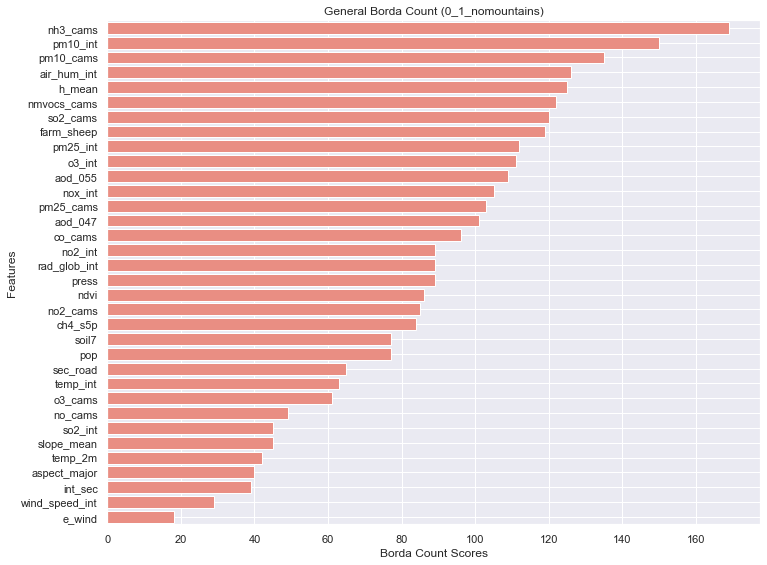
\includegraphics[scale =0.50]{images/tests/0_1_nomountainsnh3_st.png}
\caption{FS results obtained with Ammonia (NH3) as target variable with 1 Km resolution excluding mountains.}
\label{fig:fs_nh3}
\end{figure}
So overall, the results obtained in feature selection demonstrate two things.\\
First, fine particulate should be very correlated with ammonia in the manuring period (spring). Second, ammonia is strictly related to agriculture and farming activity, in accordance with previous studies.\pagebreak
\section{Data Modelling Results}
\label{sec:modelling2}
This section collected the interpretation of the ML models results, paying attention to the results achieved by the models. 
\subsection{Interpretation of validation results with ARPA sensor}
The errors obtained in the results by the validation through particle matter decrease with higher resolution.\\
Higher resolution implies a larger number of samples for training and so a better accuracy as consequence.\\
With the PM2.5 target variable at 10 km resolution, there is a lower statistical accuracy than at 1km.
With 10 km resolution MAE reaches a maximum value of 1.448 ug/m\textsuperscript{3} (Tables \ref{tab:res10km}), while for 1 km resolution it does not exceed 0.347 ug/m\textsuperscript{3} (Tables \ref{tab:res1km})
\par 
With ammonia as target variable the error are higher.
In relation to the results obtained by RF at 1 km with PM2.5 as target variables, the ones of ammonia has a MAE that has a maximum value of 0.939 ug/m\textsuperscript{3} in the September period (table \ref{tab:nh3RF})

\begin{table}[H]
\begin{tabular}{lrrrrr}
\toprule
  &  24/03-31/03 &  18/04-25/04 &  17/07-24/07 &  3/09-10/09 &  7/10-14/10 \\
\midrule
  MAE\_sensor ($\mu$g/m\textsuperscript{3}) &        1.448 &        1.093 &        0.646 &       0.898 &       0.841 \\
RMSE\_sensor ($\mu$g/m\textsuperscript{3}) &        1.940 &        1.362 &        0.868 &       1.165 &       1.080 \\
 MSE\_sensor ($\mu$g\textsuperscript{2}/m\textsuperscript{6}) &        3.772 &        1.874 &        0.776 &       1.376 &       1.197 \\
  R2\_sensor  &        0.872 &        0.766 &        0.683 &       0.870 &       0.793 \\
\bottomrule
\end{tabular}
\caption{Random Forest prediction for PM2.5 at 10 km, excluding zones with mountains.}
\label{tab:res10km}
\end{table}
\begin{table}[H]
\begin{tabular}{lrrrrr}
\toprule
  &  24/03-31/03 &  18/04-25/04 &  17/07-24/07 &  3/09-10/09 &  7/10-14/10 \\
\midrule
  MAE\_sensor ($\mu$g/m\textsuperscript{3}) &        0.347 &        0.234 &        0.156 &       0.199 &       0.146 \\
RMSE\_sensor ($\mu$g/m\textsuperscript{3}) &        0.624 &        0.392 &        0.261 &       0.327 &       0.232 \\
 MSE\_sensor ($\mu$g\textsuperscript{2}/m\textsuperscript{6}) &        0.411 &        0.158 &        0.069 &       0.113 &       0.054 \\
  R2\_sensor  &        0.990 &        0.985 &        0.982 &       0.993 &       0.991 \\
\bottomrule
\end{tabular}
\caption{Random Forest prediction for PM2.5 at 1 km, excluding zones with mountains.}
\label{tab:res1km}
\end{table}

\begin{table}[H]
\begin{tabular}{lrrrrr}
\toprule
  &  24/03-31/03 &  18/04-25/04 &  17/07-24/07 &  3/09-10/09 &  7/10-14/10 \\
\midrule
 MAE\_sensor ($\mu$g/m\textsuperscript{3}) &        0.483 &        0.280 &        0.526 &       0.939 &       0.386 \\
RMSE\_sensor ($\mu$g/m\textsuperscript{3}) &        0.993 &        0.558 &        1.184 &       2.316 &       0.860 \\
 MSE\_sensor ($\mu$g\textsuperscript{2}/m\textsuperscript{6}) &        1.199 &        0.430 &        1.556 &       6.147 &       1.121 \\
  R2\_sensor  &        0.997 &        0.992 &        0.994 &       0.987 &       0.990 \\
\bottomrule
\end{tabular}
\caption{Random Forest prediction for NH3 at 1 km, excluding zones with mountains.}
\label{tab:nh3RF}
\end{table}
\begin{table}[H]
\begin{tabular}{lrrrrr}
\toprule
  &  24/03-31/03 &  18/04-25/04 &  17/07-24/07 &  3/09-10/09 &  7/10-14/10 \\
\midrule
 MAE\_sensor ($\mu$g/m\textsuperscript{3})&        1.904 &        2.287 &        3.126 &       2.743 &       3.146 \\
RMSE\_sensor ($\mu$g/m\textsuperscript{3}) &        2.570 &        3.341 &        4.205 &       3.841 &       4.465 \\
 MSE\_sensor ($\mu$g\textsuperscript{2}/m\textsuperscript{6}) &        6.867 &       11.579 &       18.068 &      16.405 &      21.579 \\
  R2\_sensor &        0.984 &        0.800 &        0.927 &       0.965 &       0.852 \\
\bottomrule
\end{tabular}
\caption{Neural Network prediction for NH3 at 1 km, excluding zones with mountains.}
\label{tab:nh3NN}
\end{table}
This difference should be given by a different number of ground sensor measuraments of each pollutant. The size of samples of particulate matter is larger than the one for ammonia.
In the figure \ref{fig:comparison-sensors} are shown the observations at 10km resolution of each different target variable used in this case study. \\
The legend shows whether the cell has an added value by KNN or not. By these images we can observe how the number of samples passed from 28 to 173 for PM2.5 as target variable and from 8 to 69 for NH3.
\begin{figure}[H] 
    \centering
    \subfloat[PM2.5 as target variable.]{%
        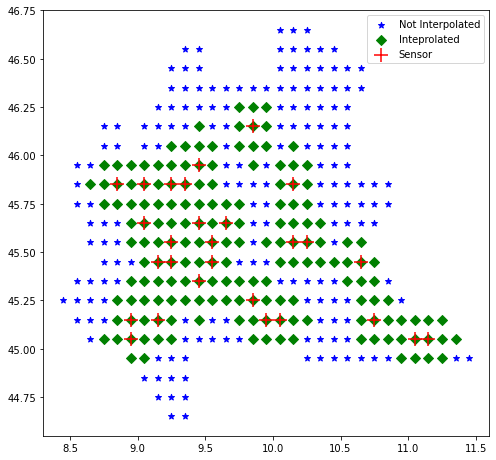
\includegraphics[width=0.5\textwidth]{images/pm25_sensors.png}%
        %
        }%
    \hfill%
    \subfloat[NH3 as target variable.]{%
        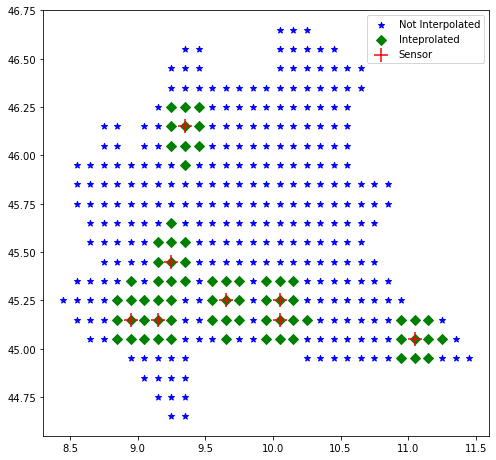
\includegraphics[width=0.5\textwidth]{images/nh3_sensors.png}%
        %
        }%
    \caption{In these images }
    \label{fig:comparison-sensors}
\end{figure}
We can observe also that generally, the Random Forest model makes more accurate predictions than the Neural Network by Keras (Tables \ref{tab:nh3RF} and \ref{tab:nh3NN}). \\
This may be since RF algorithm uses the ensemble learning method for regression, a technique that joins estimation from multiple models to have more accurate predictions than a single model.\\ 
R\textsuperscript{2} in each test assumes a positive value, meaning that the pollutants taken into consideration in this case study can be explained by the regression models. 
\pagebreak

\subsection{Importance of the FS}
The underlying tables provide model results if FS is before applied or not.

It can be observed that feature selection is meaningful for the pre-processing phase since aims at discarding eventually useless variables and taking only the ones really relevant to the target variable. \\
In the results obtained, we can detect that selection of variable with FS assume a key role for reducing the training time.\\ 
Instead, there is no visible difference in terms of accuracy in the results obtained in both resolutions (Tables \ref{fig:importance10km} and \ref{fig:importance1km}).\\
These findings suggest that if a reduction of the input variables is applyied the training will be faster without compromising its accuracy.
In conclusion, the difference between the results of this test and the ones run for each period show also the presence of overfitting in my models. Indeed, results obtained with temporal hold-out validation (in particular for  R\textsuperscript{2}) shows how the \acrshort{rf} model can't make accurate predictions about new data (which comes from a different period).  

\begin{table}[H]
\centering
\subfloat[10 km resolution.]
{\begin{tabular}{lrr}
\toprule
 &  With FS & Without FS \\
  \midrule
 MAE\_sensor ($\mu$g/m\textsuperscript{3}) &        2.123  &        2.061 \\
RMSE\_sensor ($\mu$g/m\textsuperscript{3}) &        2.645 &        2.567 \\
 MSE\_sensor ($\mu$g\textsuperscript{2}/m\textsuperscript{6}) &        6.997  &       6.592 \\
  R2\_sensor  &        0.130  &         0.176\\
   Training time (s) & 2.402 & 3.637 \\
\end{tabular}
\label{fig:importance10km}}
\\
\subfloat[1 km resolution.]
{\begin{tabular}{lrr}
\toprule
& With FS &  Without FS\\
\midrule
 MAE\_sensor ($\mu$g/m\textsuperscript{3})&        2.677 &        2.660 \\
RMSE\_sensor ($\mu$g/m\textsuperscript{3})&        3.230  &        3.252\\
 MSE\_sensor ($\mu$g\textsuperscript{2}/m\textsuperscript{6})&        10.434 &        10.575  \\
  R2\_sensor &        -0.268 &        -0.285 \\
   Training time (s) & 17.298 & 24.338 \\
 \label{fig:importance1km}
\end{tabular}}
\caption{Random Forest prediction for PM2.5, including zones with mountains using or not FS.}
\end{table}

\chapter{Conclusion}
\label{chap:conclusion}
The aim of this chapter is to highlight the main aspect that I have realized in my work.
Based on the results achieved in the previous chapter, we can conclude that Machine Learning models performed differently for many factors such as the type of model, configuration, and resolution.
In the test run before, it's possible to realize the factor that make a result more accurate than others.\\
An important aspect shown in my work is the importance of the number of ground sensor observations used from training data. In order to have enhanced estimation, reducing the lack of these is essential.\\
In ML models performance grows up as the model complexity, turning such systems into “black box” approaches and implying uncertainty in the way they work and come to decisions. 
This becomes a problematic challenge for machine learning systems to be used in critical domains, such as healthcare or the economic aspect.
The use of feature selection supports more efficient debugging for causalities and greater trust in the model.
The selection of features also attempts to clarify the decision of a model by determining the influence of each input variable. 
Scores of feature selection alone may not give a proper comprehension of the model’s reasoning, but it's partially helpful for interpreting the decisions taken.\\
Nevertheless, this case of study was not brought to build a proper model for air pollution forecast; instead it aims to detect how the selection of relevant features could affect the interpretability and the performance of the model. \\
The present study confirmed the findings about the model performance which increases if a feature selection is applied, in particular when we have to deal with limited sample of data\cite{vabalas2019machine}. 
In addition, what coming out from this is that more the training sample size is limited, more an accurate selection of the most weighted variables is needed to increase its performance.
We can say that the feature selection application is necessary but not a sufficient condition to have an increment in the model performance.
\begin{comment}
In this work, so it is highlighted the effect of how the training in ML should benefit from an accurate selection of variable. 
\end{comment}
Instead of faultless building model with exact predictions, the results in this research pointed more towards having an interpretable model from the covariates chosen. 
One of the future outcomes from this is absolutely the importance of a model sufficiently explained.
Future research on AI should extend the explanations and interpretability of ML models.
In high-risk applications, AI should not be in blind. 
It's needed to dissect a model for a proper comprehension and explanation.
For sure models like those could be helpful for the implementation of precise forecast models.  
For instance, this could be used as an important component for making average through an ensemble technique for more complex and complete model (as it has been already done with the CAMS model).
\\
Finally, this work argued that with using feature selection it's possible to detect which are the main factors affecting the target variable and, possibly, to control them such as reducing pollutants effects.\\
The score assumed by each different variable in the case of study provide a measure of the influence with respect to ammonia and fine particle formation, with also confirmation in literature.
\begin{comment}
Looking forward, further attempts for reducing pollutant formation should be made by procedures actually used.
\end{comment}


\appendix
\chapter{Appendix: comparison with CAMS model  }
\label{chap:appendixCAMS}
The comparison between the models of my results and CAMS data shows how values are very far from them. MAE for PM2.5 values is around 5 while for ammonia around 10 ug/m\textsuperscript{3}. \\
Another difference between the two models is the R\textsuperscript{2} value which assumes a negative value in most cases. It proves the presence of a big difference between training and test values. 
\begin{table}[H]
\begin{tabular}{lrrrrr}
\toprule
  &  24/03-31/03 &  18/04-25/04 &  17/07-24/07 &  3/09-10/09 &  7/10-14/10 \\
\midrule
  MAE\_cams ($\mu$g/m\textsuperscript{3})&        7.800 &        6.556 &        2.110 &       3.060 &       3.478 \\
  RMSE\_cams ($\mu$g/m\textsuperscript{3})&        9.262 &        7.571 &        2.745 &       3.623 &       4.059 \\
   MSE\_cams ($\mu$g\textsuperscript{2}/m\textsuperscript{6})&       86.279 &       57.593 &        7.548 &      13.266 &      16.591 \\
    R2\_cams &       -2.147 &       -7.492 &       -2.846 &      -0.258 &      -1.096 \\
\bottomrule
\end{tabular}
\caption{Random Forest prediction for PM2.5 at 1 km, including zones with mountains.}
\label{tab:cams1}
\end{table}
\begin{table}[H]
\begin{tabular}{lrrrrr}
\toprule
  &  24/03-31/03 &  18/04-25/04 &  17/07-24/07 &  3/09-10/09 &  7/10-14/10 \\
\midrule
   MAE\_cams ($\mu$g/m\textsuperscript{3})&       18.401 &       10.414 &       11.746 &      14.180 &      12.012 \\
  RMSE\_cams ($\mu$g/m\textsuperscript{3})&       19.196 &       12.126 &       17.744 &      21.241 &      13.697 \\
   MSE\_cams ($\mu$g\textsuperscript{2}/m\textsuperscript{6})&      368.858 &      147.652 &      323.418 &     456.145 &     188.650 \\
    R2\_cams &        0.136 &       -1.511 &       -0.158 &      -0.001 &      -0.060 \\
\bottomrule
\end{tabular}
\caption{Random Forest prediction for NH3 at 1 km, excluding zones with mountains.}
\label{tab:cams2}
\end{table}
These results are in contrast with the FS results, where the correlation between the ARPA values (target variable) and the CAMS models is one of the strongest.
From these results and the ones obtained by FS in the , we hypothesize that both pm25\_st / nh3\_st and pm25\_cams / nh3\_cams variables measure the same pollution phenomenon (figure \ref{fig:a}), but between them there would be a bias in the samples obtained (tables \ref{tab:cams1} and \ref{tab:cams2}).\\
Obviously, the model of Copernicus Atmosphere Monitoring Service provides different results than the one obtained by me, since is built very differently. CAMS is built through an ensemble median, averaged by eleven European air quality forecasting systems. Therefore, the median model should perform better than the individual model products \cite{riccio2007seeking}.
Anyway, through information collected on the Copernicus website, only a limited number of ground observations are detected in the Italian territory. 
The map in in figure \ref{fig:cams} includes a set of points layers representing the forecast performance of the station used by the ensemble median model of CAMS.
It can be seen that in Italy there is only 2 observations in Lombardy for PM2.5 detection.\\
Nothing was found for Ammonia.
\begin{figure}[H]
    \centering
    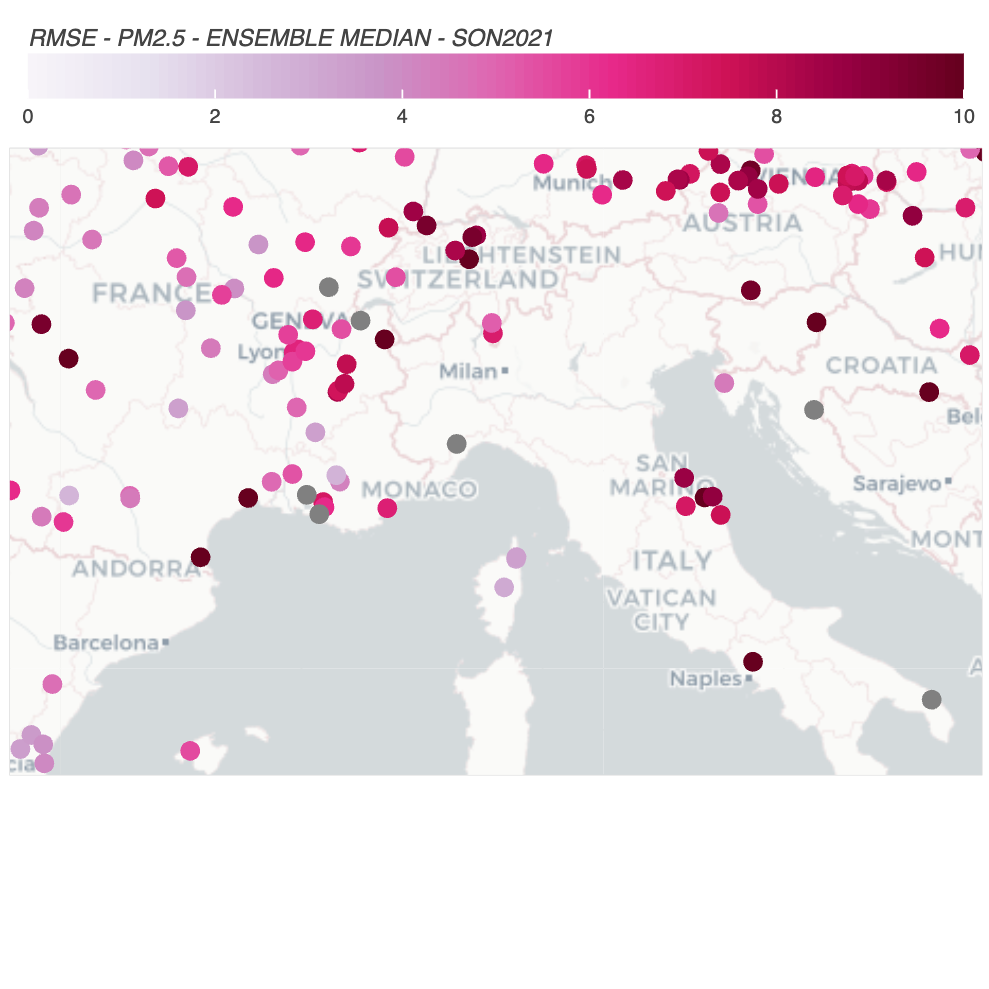
\includegraphics[scale=0.25]{images/cams_obs.png}
    \caption{Forecast performance at station and country level for the RMSE ($\mu$g/m\textsuperscript{3}) of the PM2.5 of CAMS \cite{camsobs} in 2021. 
}
    \label{fig:cams}
\end{figure}

So, by the validation results and the larger number of ground observations provided by ARPA in this data collection, we hypothesize that this model should perform better on this local scale.
\par
Based on these results, we can point out that Random Forest is more accurate than the  Neural Network model and that the performance is higher for particulate matter than ammonia estimation.\\
\begin{comment}
Random Forest indeed is one of the most preferred also in the literature prediction models for its easy configuration.
\end{comment}

\chapter{Appendix: Results}
\label{chap:appendix}
In this appendix are collected all results of
\begin{itemize}
    \item feature selection evaluated by fs\_results.ipynb;
    \item model prediction errors computed with:
    \begin{itemize}
        \item Keras\_prediction\_model.ipynb;
        \item RandomForest\_prediction\_model.ipynb;
    \end{itemize} 
    In particular, errors computed are related to:
    \begin{itemize}
        \item the validation with ARPA values (labeled with '\_sensor');
        \item the validation with CAMS values (labeled with '\-cams');
    \end{itemize}
\end{itemize}
\section{Feature Selection results}
\subsection{Borda Count results}
\begin{figure}[H]
\centering
\subfloat[10 Km resolution with mountains]{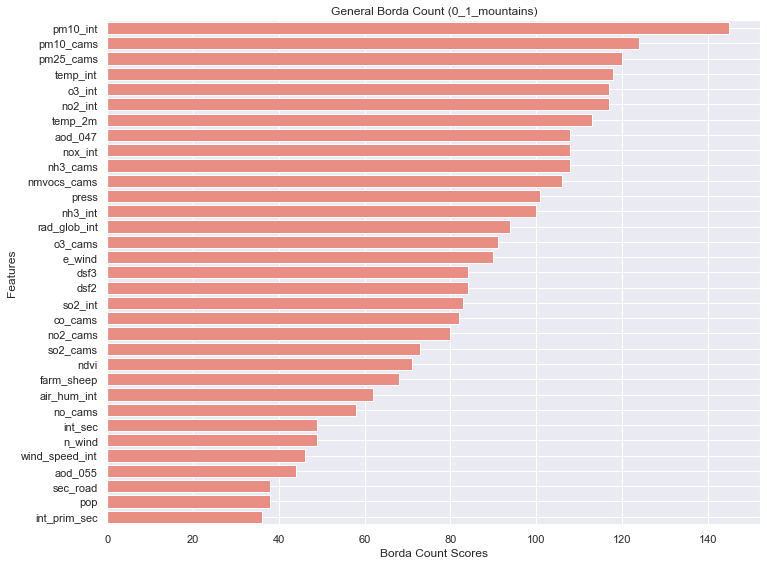
\includegraphics[scale =0.40]{images/tests/0_1_mountainspm25_st.png}}\\
\subfloat[10 Km resolution with mountains]{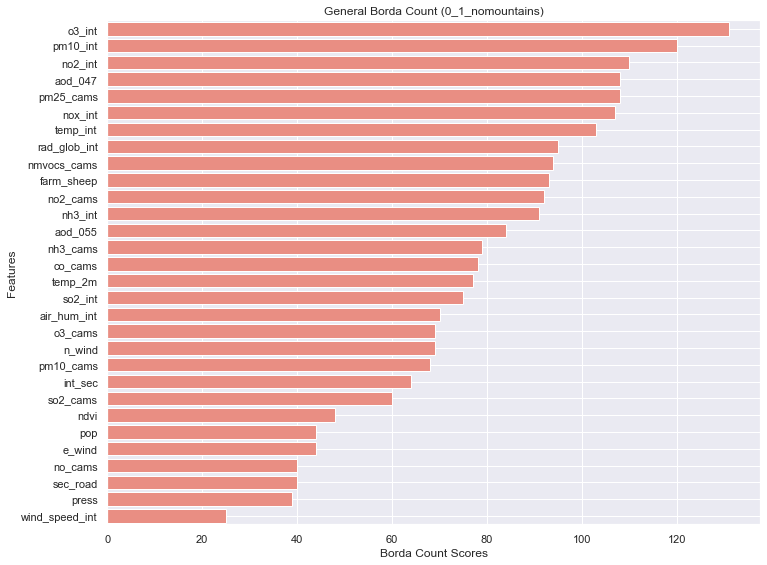
\includegraphics[scale =0.40]{images/tests/0_1_nomountainspm25_st.png}}
\caption{FS results obtained with fine particulate ('pm25\_st') as target variable and 10 km resolution. The results are averaged over the 5 periods. }
\end{figure}
\begin{figure}[H]
\centering
\subfloat[1 Km resolution with mountains]{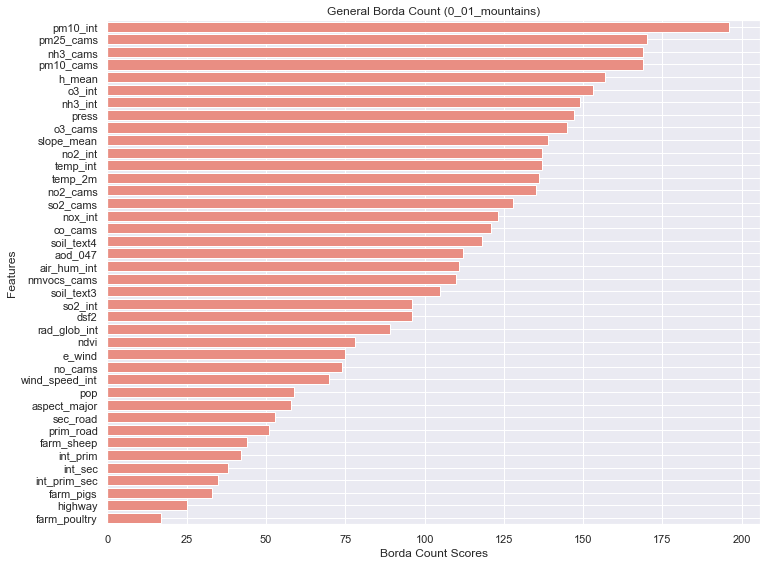
\includegraphics[scale =0.42]{images/tests/0_01_mountainspm25_st.png}}\\
\subfloat[1 Km resolution with mountains]{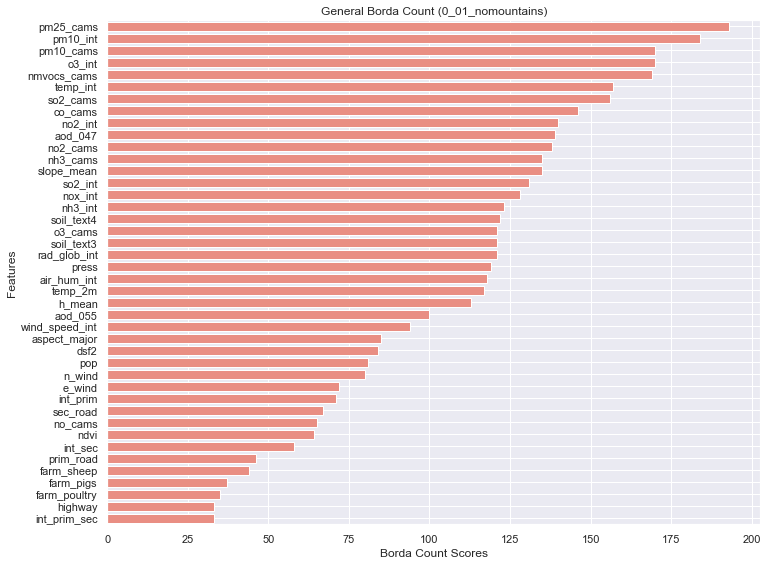
\includegraphics[scale =0.42]{images/tests/0_01_nomountainspm25_st.png}}
\caption{FS results obtained with fine particulate ('pm25\_st') as target variable and 1 km resolution. The results are averaged over the 5 periods.}
\end{figure}
\begin{figure}[H]
\centering
\subfloat[10 Km resolution with mountains]{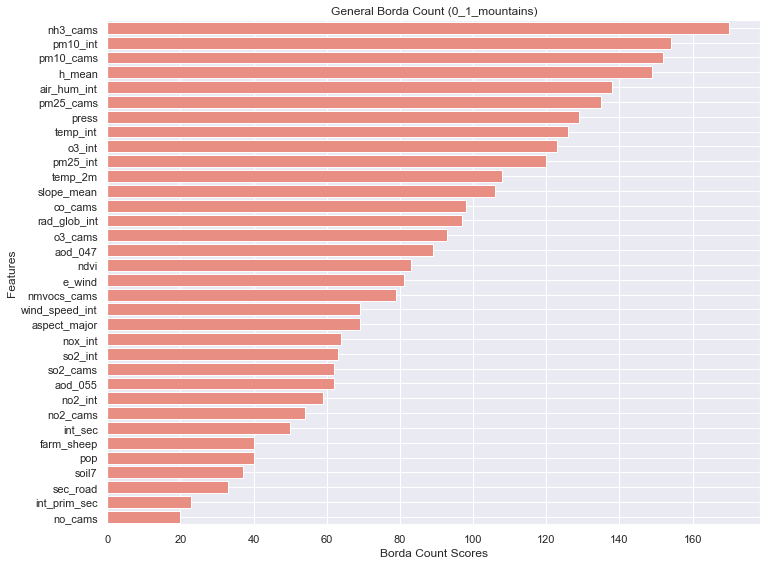
\includegraphics[scale =0.42]{images/tests/0_1_mountainsnh3_st.png}}\\
\subfloat[10 Km resolution with mountains]{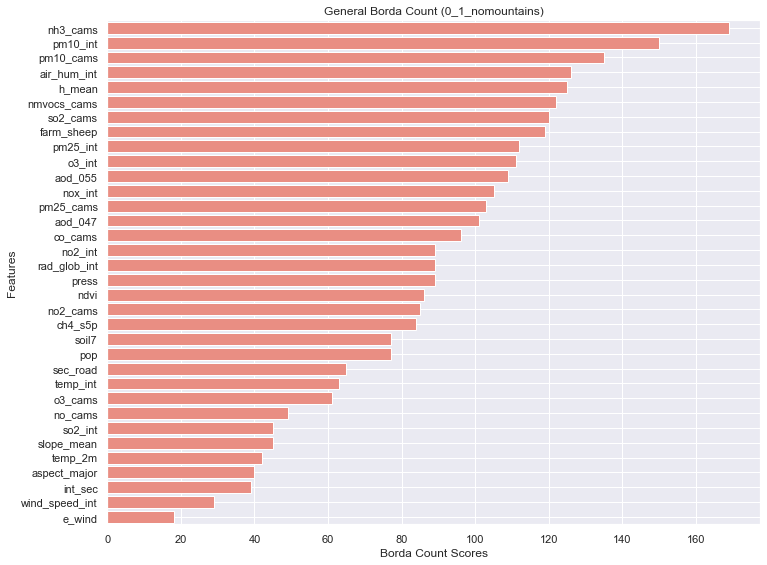
\includegraphics[scale =0.42]{images/tests/0_1_nomountainsnh3_st.png}}
\caption{FS results obtained with ammonia ('nh3\_st') as target variable and 10 km resolution. The results are averaged over the 5 periods.}
\end{figure}
\begin{figure}[H]
\centering
\subfloat[1 Km resolution with mountains]{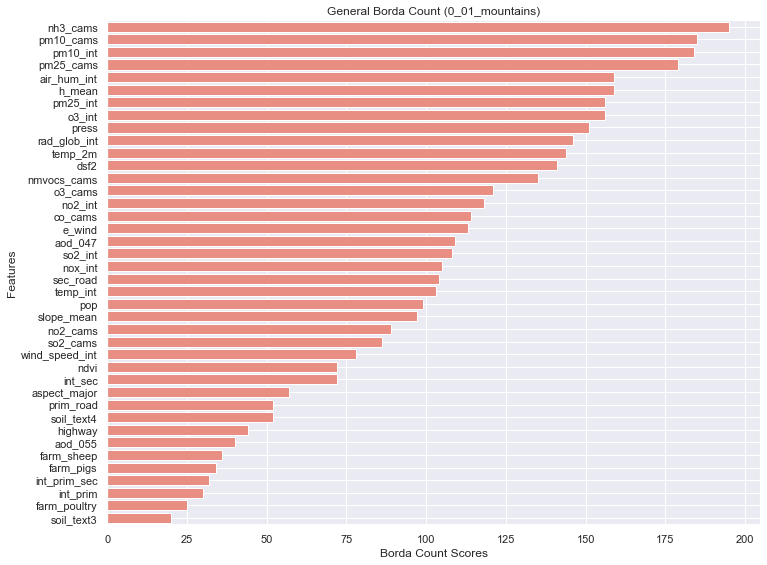
\includegraphics[scale =0.42]{images/tests/0_01_mountainsnh3_st.png}}\\
\subfloat[1 Km resolution with mountains]{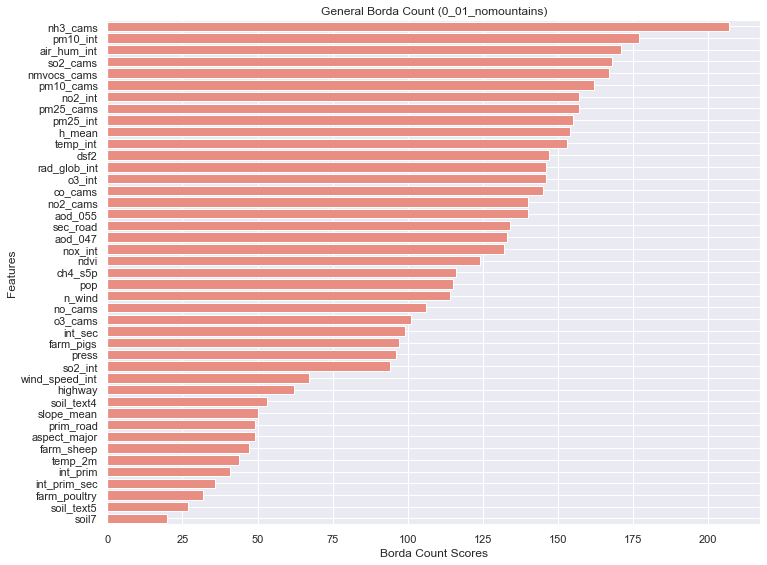
\includegraphics[scale =0.42]{images/tests/0_01_nomountainsnh3_st.png}}
\caption{FS results obtained with ammonia ('nh3\_st') as target variable and 1 km resolution. The results are averaged over the 5 periods.}
\end{figure}
\subsection{Pearson correlation index results}
\begin{figure}[H]
    \centering
    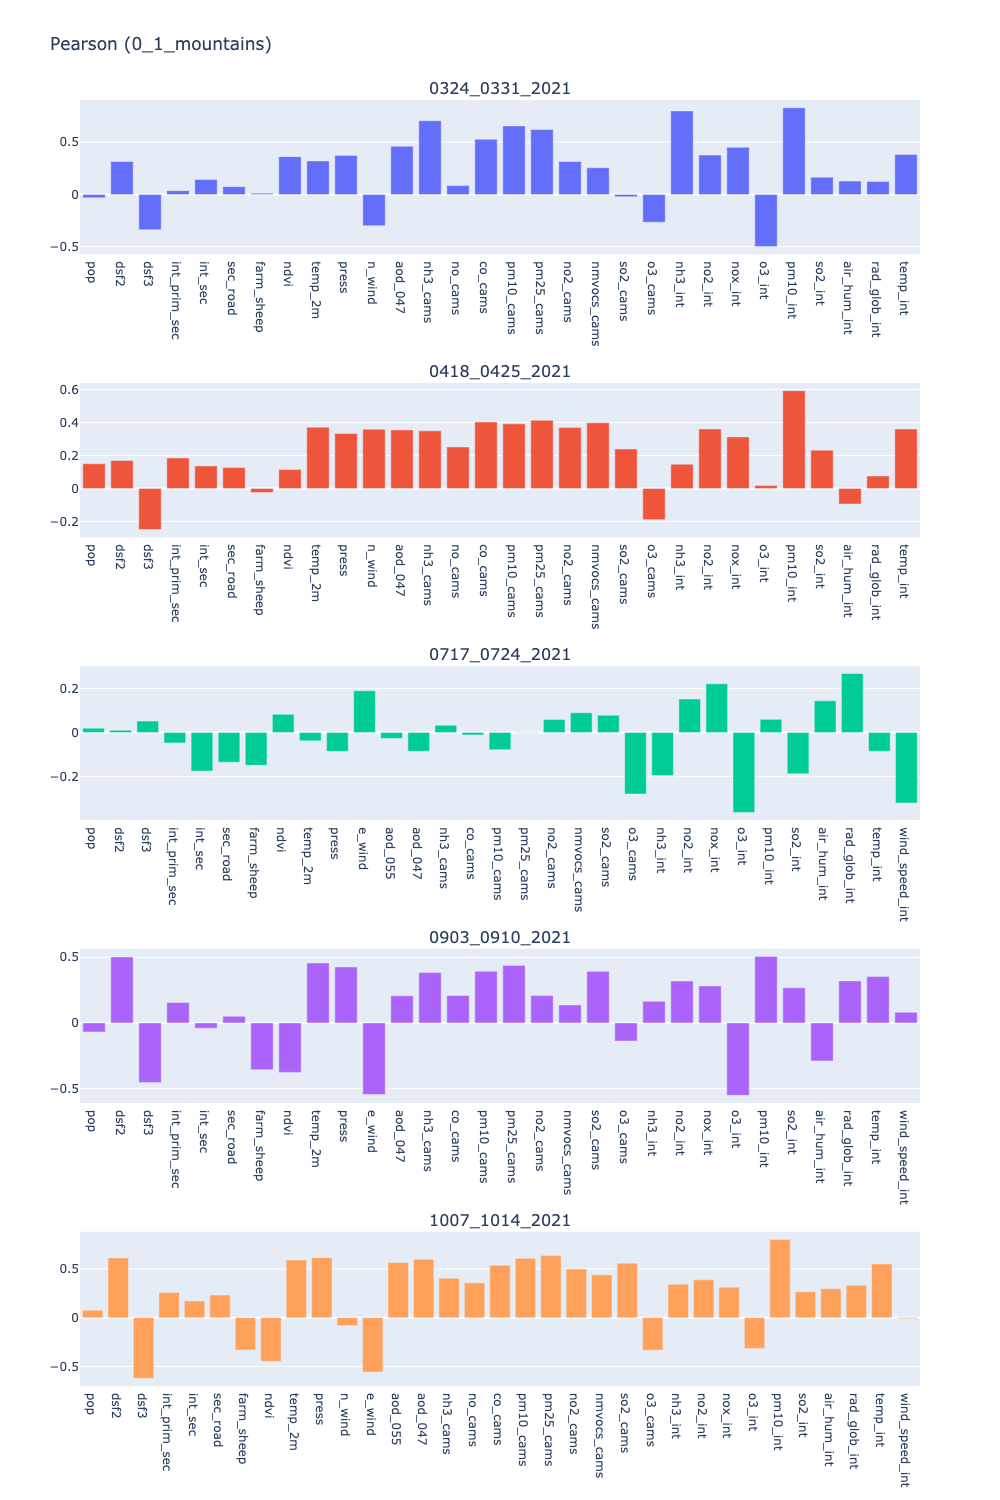
\includegraphics[scale=0.38]{images/tests/0_1_mountainspm25_st_pearson.png}
    \caption{Pearson correlation index results with respect to fine particulate ('pm25\_st') as target variable, with 10km resolution including mountains in each period. }
\end{figure}
\begin{figure}[H]
    \centering
    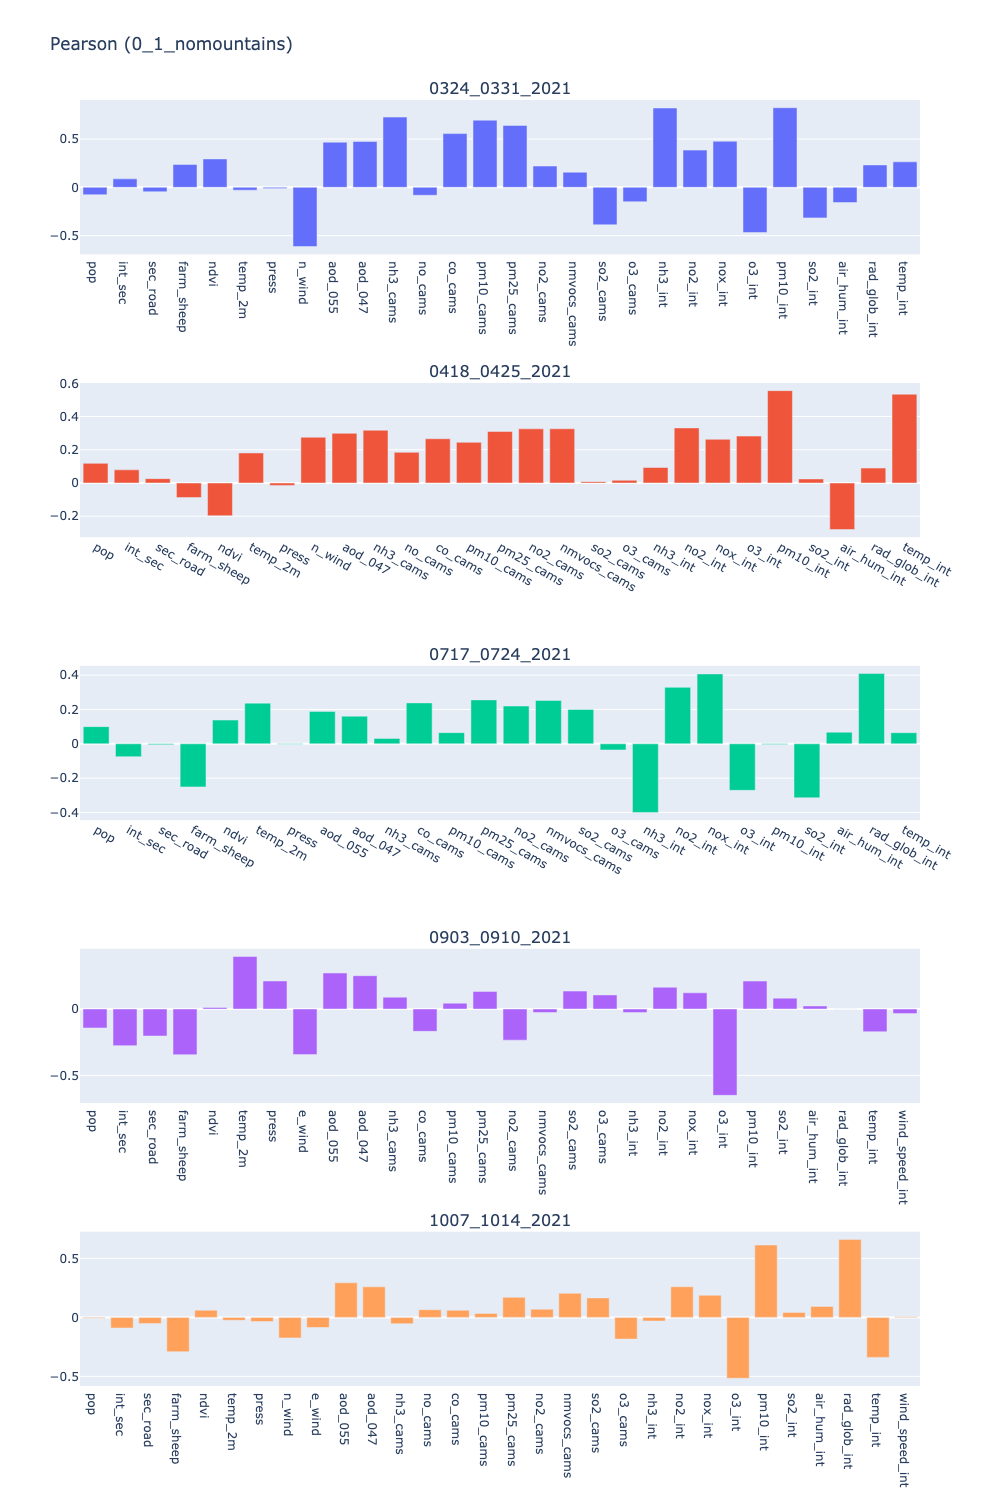
\includegraphics[scale=0.38]{images/tests/0_1_nomountainspm25_st_pearson.png}
    \caption{Pearson correlation index results with respect to fine particulate ('pm25\_st') as target variable, with 10km resolution excluding mountains in each period.}
    
\end{figure}
\begin{figure}[H]
    \centering
    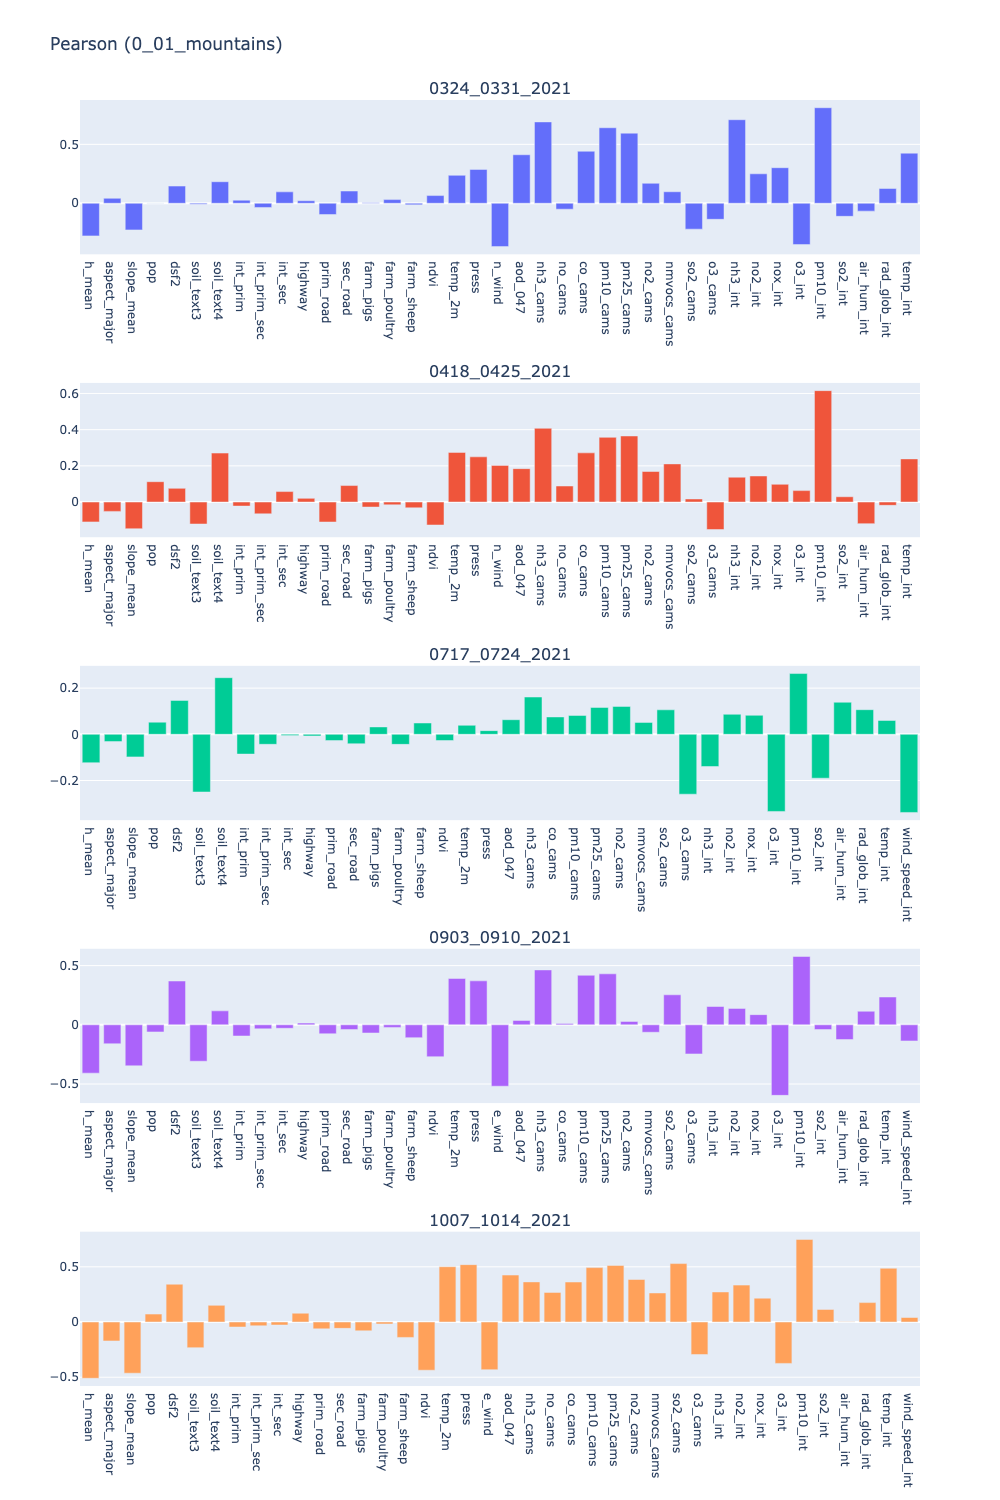
\includegraphics[scale=0.38]{images/tests/0_01_mountainspm25_st_pearson.png}
    \caption{Pearson correlation index results with respect to fine particulate ('pm25\_st') as target variable, with 1km resolution including mountains in each period.}
    
\end{figure}
\begin{figure}[H]
    \centering
    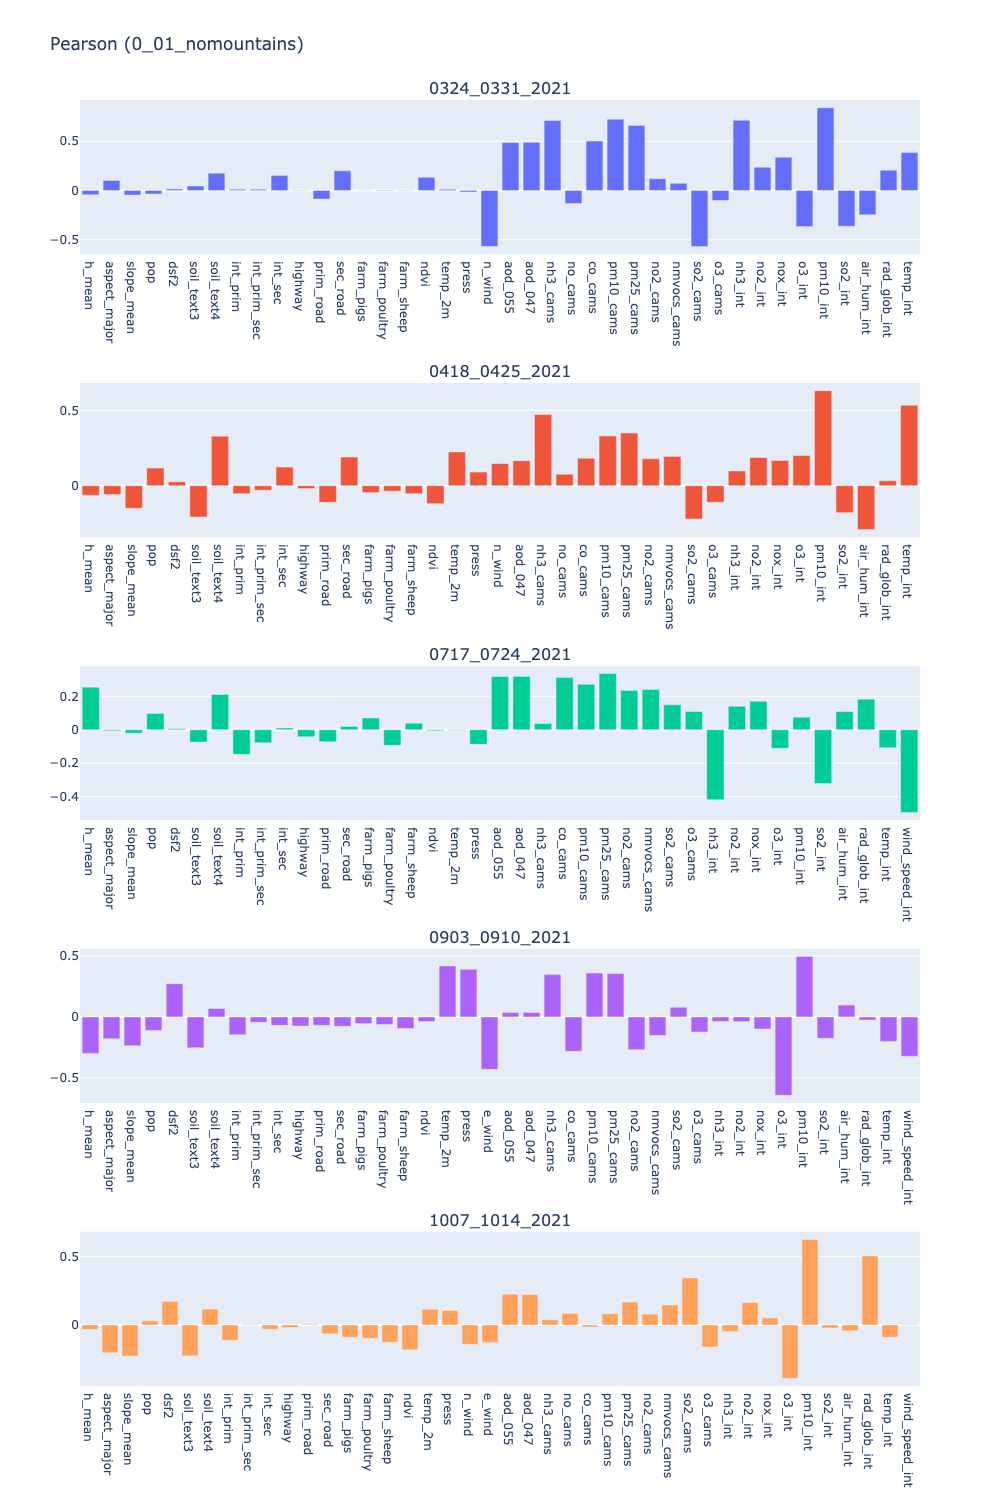
\includegraphics[scale=0.38]{images/tests/0_01_nomountainspm25_st_pearson.png}
    \caption{Pearson correlation index results with respect to fine particulate ('pm25\_st') as target variable, with 1km resolution excluding mountains in each period.}
    
\end{figure}


\begin{figure}[H]
    \centering
    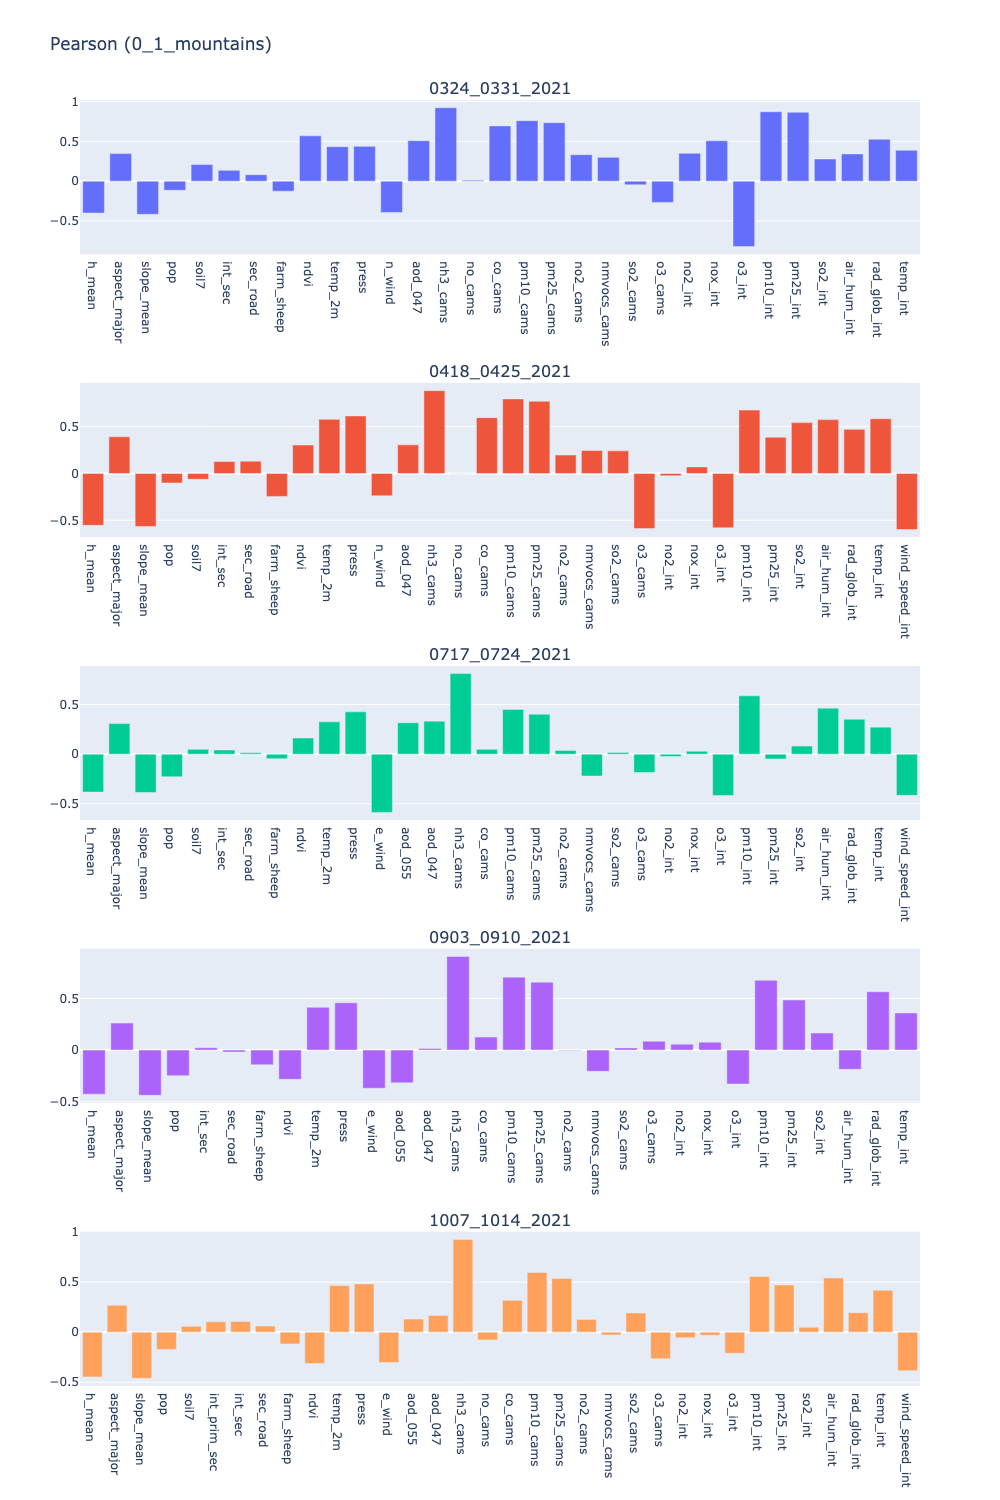
\includegraphics[scale=0.38]{images/tests/0_1_mountainsnh3_st_pearson.png}
    \caption{Pearson correlation index results with respect to ammonia ('nh3\_st') as target variable, with 10km resolution including mountains in each period.}
    
\end{figure}
\begin{figure}[H]
    \centering
    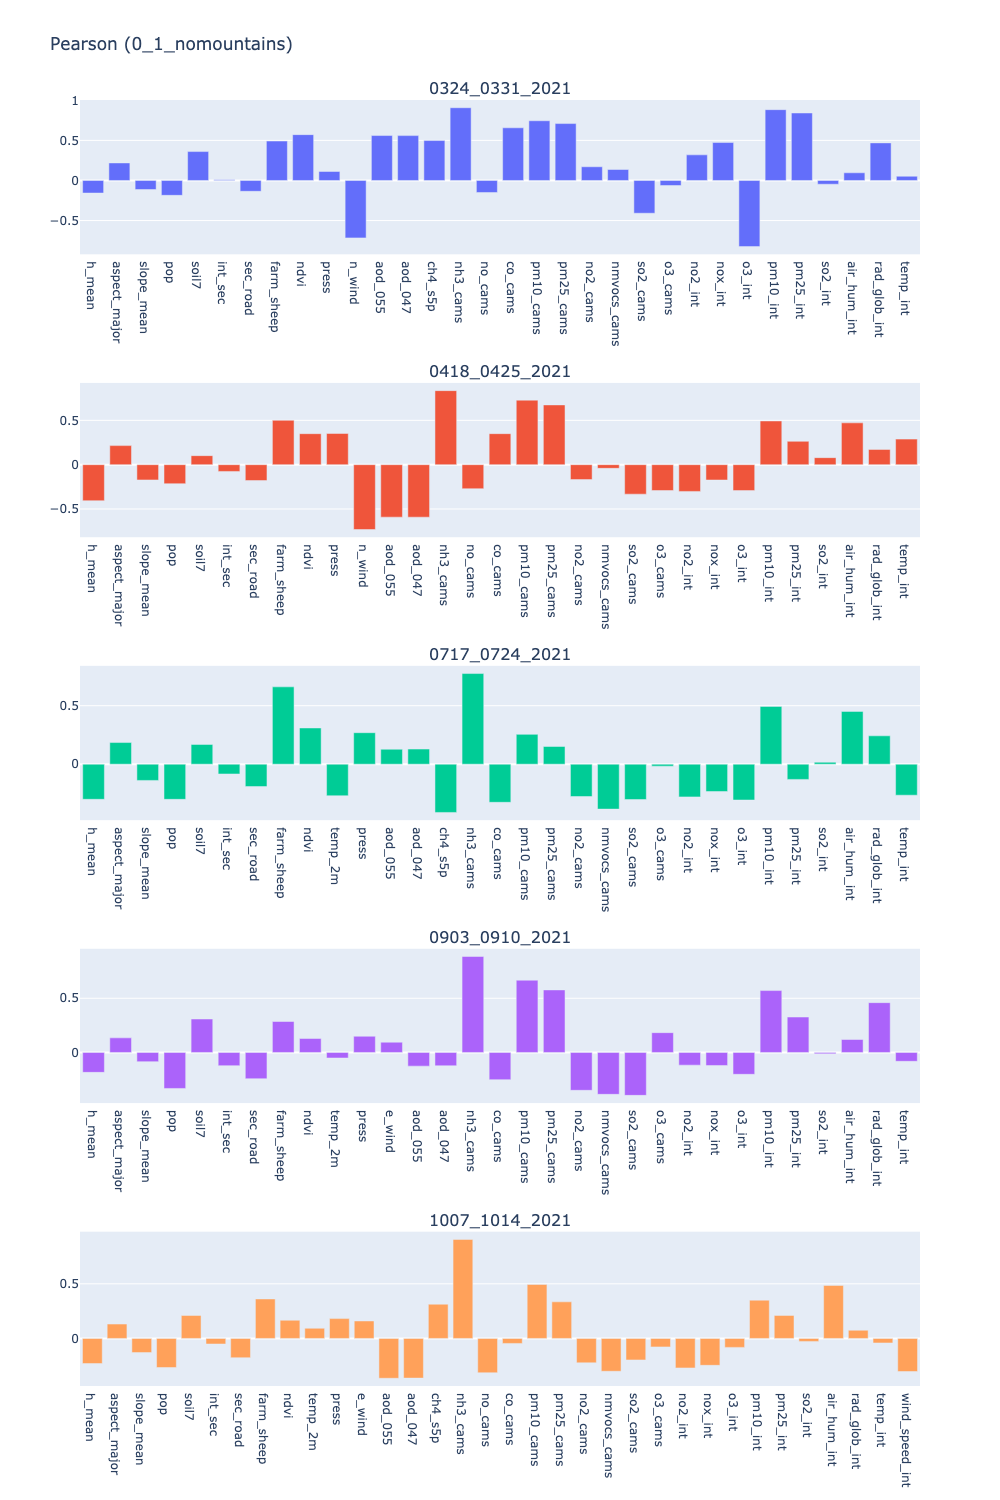
\includegraphics[scale=0.38]{images/tests/0_1_nomountainsnh3_st_pearson.png}
    \caption{Pearson correlation index results with respect to ammonia ('nh3\_st') as target variable, with 10km resolution excluding mountains in each period.}
    
\end{figure}
\begin{figure}[H]
    \centering
    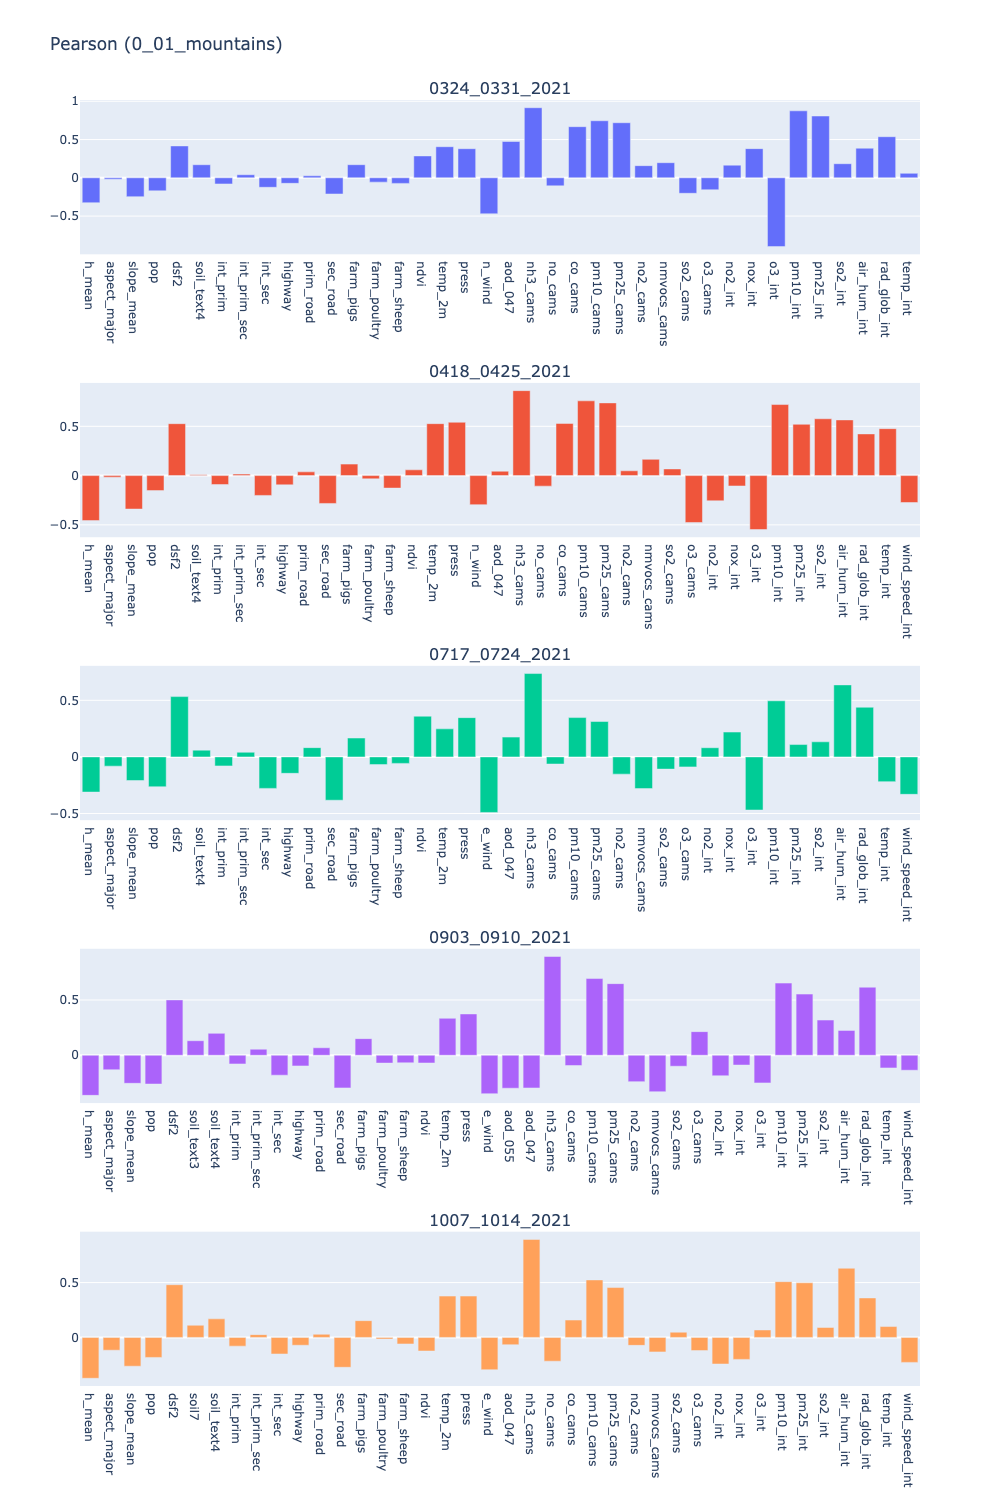
\includegraphics[scale=0.38]{images/tests/0_01_mountainsnh3_st_pearson.png}
    \caption{Pearson correlation index results with respect to ammonia ('nh3\_st') as target variable, with 1km resolution including mountains in each period.}
    
\end{figure}
\begin{figure}[H]
    \centering
    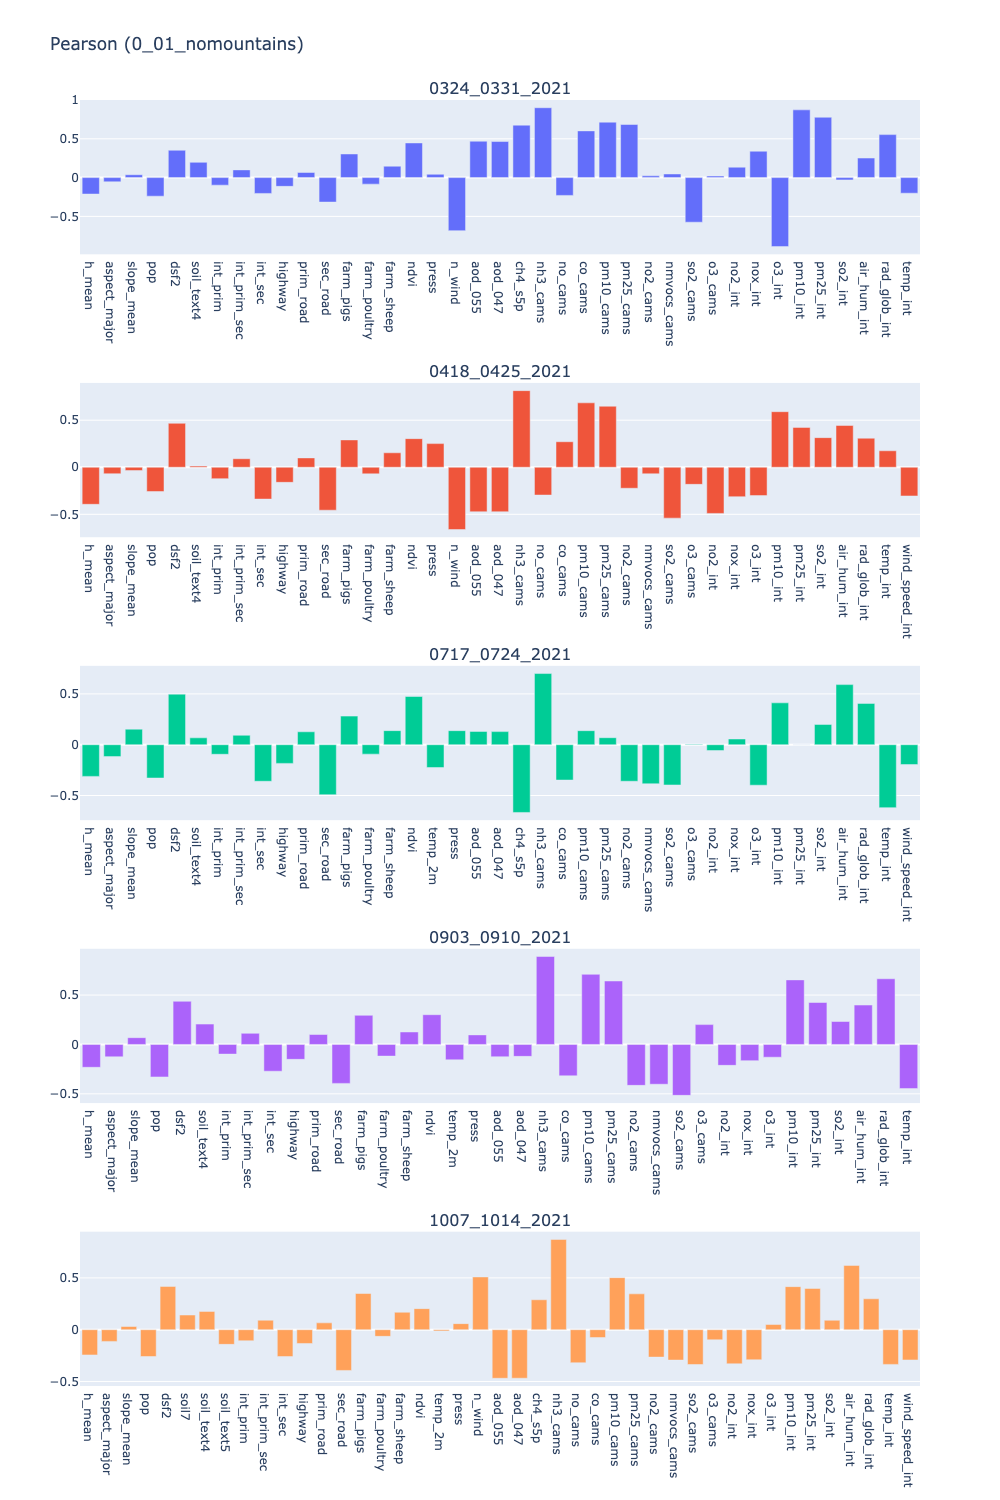
\includegraphics[scale=0.38]{images/tests/0_01_nomountainsnh3_st_pearson.png}
    \caption{Pearson correlation index results with respect to ammonia ('nh3\_st') as target variable, with 1km resolution excluding mountains in each period.}
    
\end{figure}

\section{ML models results}
\subsection{Random Forest}
\begin{table}[H]
\begin{tabular}{lrrrrr}
\toprule
 &  24/03-31/03 &  18/04-25/04 &  17/07-24/07 &  3/09-10/09 &  7/10-14/10 \\
\midrule
 MAE\_sensor ($\mu$g/m\textsuperscript{3})&        1.239 &        0.900 &        0.566 &       0.987 &       0.751 \\
RMSE\_sensor ($\mu$g/m\textsuperscript{3})&        1.768 &        1.133 &        0.745 &       1.330 &       1.013 \\
 MSE\_sensor ($\mu$g\textsuperscript{2}/m\textsuperscript{6})&        3.215 &        1.295 &        0.571 &       1.802 &       1.067 \\
  R2\_sensor &        0.883 &        0.812 &        0.722 &       0.834 &       0.858 \\
   MAE\_cams ($\mu$g/m\textsuperscript{3})&        7.800 &        6.556 &        2.110 &       3.060 &       3.478 \\
  RMSE\_cams ($\mu$g/m\textsuperscript{3})&        9.262 &        7.571 &        2.745 &       3.623 &       4.059 \\
   MSE\_cams ($\mu$g\textsuperscript{2}/m\textsuperscript{6})&       86.279 &       57.593 &        7.548 &      13.266 &      16.591 \\
    R2\_cams &       -2.147 &       -7.492 &       -2.846 &      -0.258 &      -1.096 \\
\bottomrule
\end{tabular}
\caption{Random Forest prediction for PM2.5 with 10 km resolution, including zones with mountains.}
\end{table}
\begin{table}[H]
\begin{tabular}{lrrrrr}
\toprule
 &  24/03-31/03 &  18/04-25/04 &  17/07-24/07 &  3/09-10/09 &  7/10-14/10 \\
\midrule
 MAE\_sensor ($\mu$g/m\textsuperscript{3})&        1.448 &        1.093 &        0.646 &       0.898 &       0.841 \\
RMSE\_sensor ($\mu$g/m\textsuperscript{3})&        1.940 &        1.362 &        0.868 &       1.165 &       1.080 \\
 MSE\_sensor ($\mu$g\textsuperscript{2}/m\textsuperscript{6})&        3.772 &        1.874 &        0.776 &       1.376 &       1.197 \\
  R2\_sensor &        0.872 &        0.766 &        0.683 &       0.870 &       0.793 \\
   MAE\_cams ($\mu$g/m\textsuperscript{3})&        8.230 &        7.914 &        1.386 &       3.581 &       3.744 \\
  RMSE\_cams ($\mu$g/m\textsuperscript{3})&        9.663 &        8.714 &        1.672 &       4.105 &       4.336 \\
   MSE\_cams ($\mu$g\textsuperscript{2}/m\textsuperscript{6})&       95.109 &       76.441 &        2.867 &      16.923 &      18.964 \\
    R2\_cams &       -2.312 &       -8.546 &       -0.185 &      -0.632 &      -2.373 \\
\bottomrule
\bottomrule
\end{tabular}
\caption{Random Forest prediction for PM2.5 with 10 km resolution, excluding zones with mountains.}
\end{table}
\begin{table}[H]
\begin{tabular}{lrrrrr}
\toprule
 &  24/03-31/03 &  18/04-25/04 &  17/07-24/07 &  3/09-10/09 &  7/10-14/10 \\
\midrule
 MAE\_sensor ($\mu$g/m\textsuperscript{3})&        0.251 &        0.186 &        0.147 &       0.172 &       0.132 \\
RMSE\_sensor ($\mu$g/m\textsuperscript{3})&        0.503 &        0.361 &        0.255 &       0.285 &       0.240 \\
 MSE\_sensor ($\mu$g\textsuperscript{2}/m\textsuperscript{6})&        0.283 &        0.138 &        0.066 &       0.084 &       0.059 \\
  R2\_sensor &        0.992 &        0.985 &        0.981 &       0.994 &       0.993 \\
   MAE\_cams ($\mu$g/m\textsuperscript{3})&        8.966 &        7.566 &        1.936 &       3.574 &       3.974 \\
  RMSE\_cams ($\mu$g/m\textsuperscript{3})&       10.310 &        8.472 &        2.487 &       4.099 &       4.580 \\
   MSE\_cams ($\mu$g\textsuperscript{2}/m\textsuperscript{6})&      106.414 &       71.818 &        6.213 &      16.810 &      20.988 \\
    R2\_cams &       -1.821 &       -7.099 &       -0.727 &      -0.180 &      -1.578 \\
\bottomrule
\end{tabular}
\caption{Random Forest prediction for PM2.5 with 1 km resolution, including zones with mountains.}
\end{table}
\begin{table}[H]
\begin{tabular}{lrrrrr}
\toprule
 &  24/03-31/03 &  18/04-25/04 &  17/07-24/07 &  3/09-10/09 &  7/10-14/10 \\
\midrule
 MAE\_sensor ($\mu$g/m\textsuperscript{3})&        0.347 &        0.234 &        0.156 &       0.199 &       0.146 \\
RMSE\_sensor ($\mu$g/m\textsuperscript{3})&        0.624 &        0.392 &        0.261 &       0.327 &       0.232 \\
 MSE\_sensor ($\mu$g\textsuperscript{2}/m\textsuperscript{6})&        0.411 &        0.158 &        0.069 &       0.113 &       0.054 \\
  R2\_sensor &        0.990 &        0.985 &        0.982 &       0.993 &       0.991 \\
   MAE\_cams ($\mu$g/m\textsuperscript{3})&        9.153 &        8.580 &        1.617 &       3.830 &       4.192 \\
  RMSE\_cams ($\mu$g/m\textsuperscript{3})&       10.564 &        9.294 &        1.940 &       4.382 &       4.760 \\
   MSE\_cams ($\mu$g\textsuperscript{2}/m\textsuperscript{6})&      111.721 &       86.530 &        3.766 &      19.284 &      22.676 \\
    R2\_cams &       -1.682 &       -7.131 &        0.004 &      -0.187 &      -2.674 \\
\bottomrule
\end{tabular}
\caption{Random Forest prediction for PM2.5 with 1 km resolution, excluding zones with mountains.}
\end{table}
\begin{table}[H]
\begin{tabular}{lrrrrr}
\toprule
  &  24/03-31/03 &  18/04-25/04 &  17/07-24/07 &  3/09-10/09 &  7/10-14/10 \\
\midrule
 MAE\_sensor ($\mu$g/m\textsuperscript{3})&        4.601 &        2.037 &        2.401 &       3.634 &       1.932 \\
RMSE\_sensor ($\mu$g/m\textsuperscript{3})&        5.827 &        2.809 &        3.325 &       5.074 &       2.883 \\
 MSE\_sensor ($\mu$g\textsuperscript{2}/m\textsuperscript{6})&       35.506 &        8.008 &       11.853 &      26.633 &       9.053 \\
  R2\_sensor &        0.853 &        0.815 &        0.922 &       0.854 &       0.801 \\
   MAE\_cams ($\mu$g/m\textsuperscript{3})&       14.956 &       10.748 &        8.166 &      10.326 &       9.163 \\
  RMSE\_cams ($\mu$g/m\textsuperscript{3})&       16.458 &       11.633 &       12.027 &      13.395 &      10.105 \\
   MSE\_cams ($\mu$g\textsuperscript{2}/m\textsuperscript{6})&      272.549 &      135.617 &      149.976 &     194.430 &     102.945 \\
    R2\_cams &       -0.462 &       -2.048 &        0.013 &       0.139 &      -1.066 \\
\bottomrule
\end{tabular}
\caption{Random Forest prediction for NH3 with 10 km resolution, including zones with mountains.}
\end{table}
\begin{table}[H]
\begin{tabular}{lrrrrr}
\toprule
 &  24/03-31/03 &  18/04-25/04 &  17/07-24/07 &  3/09-10/09 &  7/10-14/10 \\
\midrule
 MAE\_sensor ($\mu$g/m\textsuperscript{3})&        4.039 &        1.891 &        3.524 &       3.780 &       1.812 \\
RMSE\_sensor ($\mu$g/m\textsuperscript{3})&        5.365 &        2.496 &        4.398 &       5.358 &       2.601 \\
 MSE\_sensor ($\mu$g\textsuperscript{2}/m\textsuperscript{6})&       29.553 &        6.521 &       22.504 &      30.148 &       7.815 \\
  R2\_sensor &        0.895 &        0.829 &        0.814 &       0.848 &       0.911 \\
   MAE\_cams ($\mu$g/m\textsuperscript{3})&       15.383 &       10.758 &        8.942 &      10.304 &       9.497 \\
  RMSE\_cams ($\mu$g/m\textsuperscript{3})&       16.887 &       11.705 &       12.639 &      13.799 &      10.497 \\
   MSE\_cams ($\mu$g\textsuperscript{2}/m\textsuperscript{6})&      288.521 &      138.082 &      178.690 &     211.569 &     110.820 \\
    R2\_cams &       -0.022 &       -2.954 &       -0.236 &       0.062 &      -0.547 \\
\bottomrule
\end{tabular}
\caption{Random Forest prediction for NH3 with 10 km resolution, excluding zones with mountains.}
\end{table}
\begin{table}[H]
\begin{tabular}{lrrrrr}
\toprule
 &  24/03-31/03 &  18/04-25/04 &  17/07-24/07 &  3/09-10/09 &  7/10-14/10 \\
\midrule
 MAE\_sensor ($\mu$g/m\textsuperscript{3})&        0.450 &        0.180 &        0.505 &       0.669 &       0.345 \\
RMSE\_sensor ($\mu$g/m\textsuperscript{3})&        0.954 &        0.327 &        1.120 &       1.803 &       0.785 \\
 MSE\_sensor ($\mu$g\textsuperscript{2}/m\textsuperscript{6})&        1.065 &        0.147 &        1.861 &       4.244 &       0.732 \\
  R2\_sensor &        0.998 &        0.998 &        0.994 &       0.990 &       0.995 \\
   MAE\_cams ($\mu$g/m\textsuperscript{3})&       17.694 &       10.536 &       11.049 &      13.329 &      11.480 \\
  RMSE\_cams ($\mu$g/m\textsuperscript{3})&       18.513 &       12.046 &       16.887 &      19.503 &      12.945 \\
   MSE\_cams ($\mu$g\textsuperscript{2}/m\textsuperscript{6})&      343.112 &      145.433 &      287.761 &     382.879 &     169.030 \\
    R2\_cams &        0.227 &       -1.134 &       -0.044 &       0.124 &      -0.030 \\
\bottomrule
\end{tabular}
\caption{Random Forest prediction for NH3 with 1 km resolution, including zones with mountains.}
\end{table}
\begin{table}[H]
\begin{tabular}{lrrrrr}
\toprule
 &  24/03-31/03 &  18/04-25/04 &  17/07-24/07 &  3/09-10/09 &  7/10-14/10 \\
\midrule
 MAE\_sensor ($\mu$g/m\textsuperscript{3})&        0.483 &        0.280 &        0.526 &       0.939 &       0.386 \\
RMSE\_sensor ($\mu$g/m\textsuperscript{3})&        0.993 &        0.558 &        1.184 &       2.316 &       0.860 \\
 MSE\_sensor ($\mu$g\textsuperscript{2}/m\textsuperscript{6})&        1.199 &        0.430 &        1.556 &       6.147 &       1.121 \\
  R2\_sensor &        0.997 &        0.992 &        0.994 &       0.987 &       0.990 \\
   MAE\_cams ($\mu$g/m\textsuperscript{3})&       18.401 &       10.414 &       11.746 &      14.180 &      12.012 \\
  RMSE\_cams ($\mu$g/m\textsuperscript{3})&       19.196 &       12.126 &       17.744 &      21.241 &      13.697 \\
   MSE\_cams ($\mu$g\textsuperscript{2}/m\textsuperscript{6})&      368.858 &      147.652 &      323.418 &     456.145 &     188.650 \\
    R2\_cams &        0.136 &       -1.511 &       -0.158 &      -0.001 &      -0.060 \\
\bottomrule
\end{tabular}
\caption{Random Forest prediction for NH3 with 1 km resolution, excluding zones with mountains.}
\end{table}
\subsection{Neural Network by Keras}
\begin{table}[H]
\begin{tabular}{lrrrrr}
\toprule
 &  24/03-31/03 &  18/04-25/04 &  17/07-24/07 &  3/09-10/09 &  7/10-14/10 \\
\midrule
 MAE\_sensor ($\mu$g/m\textsuperscript{3})&        2.127 &        1.581 &        0.847 &       1.516 &       1.268 \\
RMSE\_sensor ($\mu$g/m\textsuperscript{3})&        2.643 &        2.008 &        1.046 &       1.912 &       1.591 \\
 MSE\_sensor ($\mu$g\textsuperscript{2}/m\textsuperscript{6})&        7.097 &        4.064 &        1.108 &       3.743 &       2.578 \\
  R2\_sensor &        0.750 &        0.358 &        0.408 &       0.649 &       0.672 \\
   MAE\_cams ($\mu$g/m\textsuperscript{3})&        7.800 &        6.554 &        2.113 &       3.060 &       3.478 \\
  RMSE\_cams ($\mu$g/m\textsuperscript{3})&        9.262 &        7.571 &        2.720 &       3.598 &       4.067 \\
   MSE\_cams ($\mu$g\textsuperscript{2}/m\textsuperscript{6})&       86.279 &       57.562 &        7.565 &      13.266 &      16.591 \\
    R2\_cams &       -2.147 &       -8.102 &       -3.386 &      -0.239 &      -1.158 \\
\bottomrule
\end{tabular}
\caption{Neural Network prediction for PM2.5 with 10 km resolution, including zones with mountains.}
\end{table}
\begin{table}[H]
\begin{tabular}{lrrrrr}
\toprule
 &  24/03-31/03 &  18/04-25/04 &  17/07-24/07 &  3/09-10/09 &  7/10-14/10 \\
\midrule
 MAE\_sensor ($\mu$g/m\textsuperscript{3})&        1.864 &        1.605 &        0.871 &       1.308 &       1.052 \\
RMSE\_sensor ($\mu$g/m\textsuperscript{3})&        2.257 &        1.955 &        1.100 &       1.612 &       1.327 \\
 MSE\_sensor ($\mu$g\textsuperscript{2}/m\textsuperscript{6})&        5.188 &        3.894 &        1.279 &       2.696 &       1.890 \\
  R2\_sensor &        0.826 &        0.538 &        0.457 &       0.731 &       0.653 \\
   MAE\_cams ($\mu$g/m\textsuperscript{3})&        8.243 &        7.907 &        1.383 &       3.581 &       3.744 \\
  RMSE\_cams ($\mu$g/m\textsuperscript{3})&        9.717 &        8.713 &        1.677 &       4.086 &       4.342 \\
   MSE\_cams ($\mu$g\textsuperscript{2}/m\textsuperscript{6})&       95.313 &       76.364 &        2.859 &      16.923 &      18.964 \\
    R2\_cams &       -2.281 &       -8.213 &       -0.193 &      -0.561 &      -2.351 \\
\bottomrule
\end{tabular}
\caption{Neural Network prediction for PM2.5 with 10 km resolution, excluding zones with mountains.}
\end{table}
\begin{table}[H]
\begin{tabular}{lrrrrr}
\toprule
 &  24/03-31/03 &  18/04-25/04 &  17/07-24/07 &  3/09-10/09 &  7/10-14/10 \\
\midrule
 MAE\_sensor ($\mu$g/m\textsuperscript{3})&        1.546 &        0.970 &        0.721 &       1.170 &       1.040 \\
RMSE\_sensor ($\mu$g/m\textsuperscript{3})&        1.997 &        1.340 &        0.988 &       1.528 &       1.325 \\
 MSE\_sensor ($\mu$g\textsuperscript{2}/m\textsuperscript{6})&        4.079 &        1.831 &        0.991 &       2.339 &       1.776 \\
  R2\_sensor &        0.891 &        0.798 &        0.727 &       0.839 &       0.779 \\
   MAE\_cams ($\mu$g/m\textsuperscript{3})&        8.966 &        7.567 &        1.936 &       3.574 &       3.974 \\
  RMSE\_cams ($\mu$g/m\textsuperscript{3})&       10.314 &        8.473 &        2.490 &       4.096 &       4.579 \\
   MSE\_cams ($\mu$g\textsuperscript{2}/m\textsuperscript{6})&      106.423 &       71.820 &        6.214 &      16.811 &      20.987 \\
    R2\_cams &       -1.840 &       -6.979 &       -0.735 &      -0.157 &      -1.585 \\
\bottomrule
\end{tabular}
\caption{Neural Network prediction for PM2.5 with 1 km resolution, including zones with mountains.}
\end{table}
\begin{table}[H]
\begin{tabular}{lrrrrr}
\toprule
 &  24/03-31/03 &  18/04-25/04 &  17/07-24/07 &  3/09-10/09 &  7/10-14/10 \\
\midrule
 MAE\_sensor ($\mu$g/m\textsuperscript{3})&        1.508 &        0.875 &        0.739 &       0.793 &       0.593 \\
RMSE\_sensor ($\mu$g/m\textsuperscript{3})&        1.995 &        1.174 &        0.972 &       1.002 &       0.836 \\
 MSE\_sensor ($\mu$g\textsuperscript{2}/m\textsuperscript{6})&        4.033 &        1.396 &        0.967 &       1.050 &       0.704 \\
  R2\_sensor &        0.904 &        0.868 &        0.737 &       0.937 &       0.888 \\
   MAE\_cams ($\mu$g/m\textsuperscript{3})&        9.153 &        8.581 &        1.617 &       3.830 &       4.192 \\
  RMSE\_cams ($\mu$g/m\textsuperscript{3})&       10.565 &        9.298 &        1.939 &       4.386 &       4.761 \\
   MSE\_cams ($\mu$g\textsuperscript{2}/m\textsuperscript{6})&      111.720 &       86.539 &        3.766 &      19.282 &      22.673 \\
    R2\_cams &       -1.627 &       -7.082 &       -0.006 &      -0.181 &      -2.616 \\
\bottomrule
\end{tabular}
\caption{Neural Network prediction for PM2.5 with 1 km resolution, excluding zones with mountains.}
\end{table}
\begin{table}[H]
\begin{tabular}{lrrrrr}
\toprule
 &  24/03-31/03 &  18/04-25/04 &  17/07-24/07 &  3/09-10/09 &  7/10-14/10 \\
\midrule
 MAE\_sensor ($\mu$g/m\textsuperscript{3})&        5.441 &        2.433 &        4.971 &       5.729 &       3.219 \\
RMSE\_sensor ($\mu$g/m\textsuperscript{3})&        6.896 &        3.283 &        7.496 &       7.618 &       4.613 \\
 MSE\_sensor ($\mu$g\textsuperscript{2}/m\textsuperscript{6})&       49.263 &       11.191 &       60.601 &      70.032 &      21.714 \\
  R2\_sensor &        0.785 &        0.722 &        0.618 &       0.726 &       0.722 \\
   MAE\_cams ($\mu$g/m\textsuperscript{3})&        6.660 &        4.050 &        7.537 &       6.583 &       2.601 \\
  RMSE\_cams ($\mu$g/m\textsuperscript{3})&        8.289 &        5.473 &       10.610 &       9.773 &       3.662 \\
   MSE\_cams ($\mu$g\textsuperscript{2}/m\textsuperscript{6})&       69.718 &       31.198 &      115.937 &     102.716 &      13.809 \\
    R2\_cams &        0.680 &        0.217 &        0.212 &       0.546 &       0.822 \\
\bottomrule
\end{tabular}
\caption{Neural Network prediction for NH3 with 10 km resolution, including zones with mountains.}
\end{table}
\begin{table}[H]
\begin{tabular}{lrrrrr}
\toprule
 &  24/03-31/03 &  18/04-25/04 &  17/07-24/07 &  3/09-10/09 &  7/10-14/10 \\
\midrule
 MAE\_sensor ($\mu$g/m\textsuperscript{3})&        4.625 &        2.297 &        4.749 &       5.573 &       3.139 \\
RMSE\_sensor ($\mu$g/m\textsuperscript{3})&        5.405 &        2.988 &        5.801 &       7.571 &       4.557 \\
 MSE\_sensor ($\mu$g\textsuperscript{2}/m\textsuperscript{6})&       33.849 &        9.630 &       37.672 &      58.766 &      25.848 \\
  R2\_sensor &        0.867 &        0.710 &        0.702 &       0.704 &       0.675 \\
   MAE\_cams ($\mu$g/m\textsuperscript{3})&        7.283 &        4.559 &        8.412 &       7.581 &       3.033 \\
  RMSE\_cams ($\mu$g/m\textsuperscript{3})&        8.867 &        6.016 &       11.236 &      10.874 &       4.072 \\
   MSE\_cams ($\mu$g\textsuperscript{2}/m\textsuperscript{6})&       78.979 &       36.499 &      135.704 &     123.934 &      16.818 \\
    R2\_cams &        0.710 &       -0.106 &       -0.034 &       0.425 &       0.591 \\
\bottomrule
\end{tabular}
\caption{Neural Network prediction for NH3 with 10 km resolution, excluding zones with mountains.}
\end{table}
\begin{table}[H]
\begin{tabular}{lrrrrr}
\toprule
 &  24/03-31/03 &  18/04-25/04 &  17/07-24/07 &  3/09-10/09 &  7/10-14/10 \\
\midrule
 MAE\_sensor ($\mu$g/m\textsuperscript{3})&        3.064 &        1.920 &        4.194 &       2.612 &       2.140 \\
RMSE\_sensor ($\mu$g/m\textsuperscript{3})&        3.953 &        3.010 &        5.592 &       3.497 &       2.518 \\
 MSE\_sensor ($\mu$g\textsuperscript{2}/m\textsuperscript{6})&       17.004 &        9.733 &       31.882 &      12.736 &       8.747 \\
  R2\_sensor &        0.962 &        0.861 &        0.879 &       0.968 &       0.953 \\
   MAE\_cams ($\mu$g/m\textsuperscript{3})&        8.197 &        4.031 &       10.073 &       9.247 &       4.327 \\
  RMSE\_cams ($\mu$g/m\textsuperscript{3})&       10.860 &        6.169 &       14.998 &      15.436 &       7.145 \\
   MSE\_cams ($\mu$g\textsuperscript{2}/m\textsuperscript{6})&      118.847 &       38.357 &      225.879 &     243.268 &      51.953 \\
    R2\_cams &        0.736 &        0.456 &        0.180 &       0.445 &       0.695 \\
\bottomrule
\end{tabular}
\caption{Neural Network prediction for NH3 with 1 km resolution, including zones with mountains.}
\end{table}


\begin{table}[H]
\begin{tabular}{lrrrrr}
\toprule
 &  24/03-31/03 &  18/04-25/04 &  17/07-24/07 &  3/09-10/09 &  7/10-14/10 \\
\midrule
 MAE\_sensor ($\mu$g/m\textsuperscript{3})&        1.904 &        2.287 &        3.126 &       2.743 &       3.146 \\
RMSE\_sensor ($\mu$g/m\textsuperscript{3})&        2.570 &        3.341 &        4.205 &       3.841 &       4.465 \\
 MSE\_sensor ($\mu$g\textsuperscript{2}/m\textsuperscript{6})&        6.867 &       11.579 &       18.068 &      16.405 &      21.579 \\
  R2\_sensor &        0.984 &        0.800 &        0.927 &       0.965 &       0.852 \\
   MAE\_cams ($\mu$g/m\textsuperscript{3})&        9.253 &        4.560 &       11.334 &      11.259 &       5.461 \\
  RMSE\_cams ($\mu$g/m\textsuperscript{3})&       11.641 &        6.600 &       15.831 &      17.476 &       8.145 \\
   MSE\_cams ($\mu$g\textsuperscript{2}/m\textsuperscript{6})&      135.675 &       43.816 &      257.910 &     306.085 &      67.695 \\
    R2\_cams &        0.692 &        0.254 &        0.058 &       0.342 &       0.631 \\
\bottomrule
\end{tabular}
\caption{Neural Network prediction for NH3 with 1 km resolution, excluding zones with mountains.}
\end{table}












\bibliographystyle{plain}
\bibliography{mybib.bib}       

\end{document}